\RequirePackage[l2tabu, orthodox]{nag}

%\documentclass[]{article}
\documentclass[11pt]{scrartcl}
\usepackage[usename, dvipsnames]{xcolor}
\usepackage[pdfencoding=auto]{hyperref}
\usepackage[msc-links]{amsrefs}
\usepackage{cleveref} % use \cref{}, automatically deduces theorem, proposition, etc
\usepackage[mathletters]{ucs}
\usepackage[utf8]{inputenc}
\usepackage[T1]{fontenc}
\usepackage{datetime}

\usepackage{array}
\usepackage{mathtools}
\usepackage{amsmath, amsthm, amssymb, amsfonts, amsxtra, amscd, thmtools}
\let\proof\relax
\let\endproof\relax

% Boxes around theorem environments.
\usepackage[many]{tcolorbox}

\usepackage{color}
%\usepackage{unicode-math}
\usepackage{newunicodechar}
\newunicodechar{ε}{\varepsilon}
\newunicodechar{δ}{\delta}
\newunicodechar{µ}{\mu}
\newunicodechar{→}{\to}
\newunicodechar{≤}{\leq}
\newunicodechar{∈}{\in}
\newunicodechar{⊆}{\subseteq}
\newunicodechar{Λ}{\Lambda}
\newunicodechar{∞}{\infty}
\newunicodechar{×}{\times}
\everymath{\displaystyle}



\usepackage{microtype}
\usepackage[pdfencoding=auto]{hyperref}
\usepackage{bookmark}
\usepackage{booktabs}
\usepackage{todonotes}
\usepackage[msc-links]{amsrefs}
\usepackage{cleveref} % use \cref{}, automatically deduces theorem, proposition, etc
\usepackage{csquotes}
\usepackage{longtable}
\usepackage{tabularx}
\usepackage{bbm}
% Creating multiple types of index
\usepackage{imakeidx}

% Remove indentation for new paragraphs
\usepackage{parskip}
% But leave space before amsthm environments
\makeatletter
\def\thm@space@setup{%
  \thm@preskip=2em
  \thm@postskip=2em
}
\makeatother


\usepackage{stmaryrd}
\usepackage{adjustbox}
\usepackage{centernot}
% \centernot\whatever


% Better indicator function
\usepackage{bbm}
\newcommand{\indic}[1]{\mathbbm{1} \left[ {#1} \right] }

% Highlight quote
\usepackage{environ}
\definecolor{camel}{rgb}{0.76, 0.6, 0.42}
\definecolor{babyblue}{rgb}{0.54, 0.81, 0.94}
\definecolor{block-gray}{gray}{0.85}
\NewEnviron{myblock}
{\colorbox{block-gray}{%
\parbox{\dimexpr\linewidth-2\fboxsep\relax}{%
\small\addtolength{\leftskip}{10mm}
\addtolength{\rightskip}{10mm}
\BODY}}
}
\renewcommand{\quote}{\myblock}
\renewcommand{\endquote}{\endmyblock}

% Nice math font that journals use
%\usepackage[lite]{mtpro2}
%\usepackage{mathrsfs}
%\usepackage{mathptmx}
\usepackage{lmodern}
%\usepackage[sc]{mathpazo}

% Theorem Styles
\usepackage[framemethod=tikz]{mdframed}

\theoremstyle{definition}
\newtheorem{exercise}{Exercise}[section]
\newtheorem{solution}{Solution}

% Theorem Style
\newtheoremstyle{theorem}% name
  {0em}%         Space above, empty = `usual value'
  {1em}%         Space below
  {\normalfont}% Body font
  {\parindent}%         Indent amount (empty = no indent, \parindent = para indent)
  {\bfseries}% Thm head font
  {.}%        Punctuation after thm head
  {\newline}% Space after thm head: \newline = linebreak
  {\thmname{#1}\thmnumber{ #2}\thmnote{\itshape{(#3)}}}%
\theoremstyle{theorem}
\tcolorboxenvironment{theorem}{
  boxrule=0pt,
  boxsep=0pt,
  breakable,
  enhanced jigsaw,
  fonttitle={\large\bfseries},
  opacityback=0.8,
  colframe=cyan,
  borderline west={4pt}{0pt}{orange},
  attach title to upper={}
}
\newtheorem{theorem}{Theorem}[section]

% Proposition Style
\tcolorboxenvironment{proposition}{
  boxrule=1pt,
  boxsep=0pt,
  breakable,
  enhanced jigsaw,
  opacityback=0.0,
  colframe=cyan
}
\newtheorem{proposition}[theorem]{Proposition}
\tcolorboxenvironment{lemma}{
  boxrule=1pt,
  boxsep=0pt,
  breakable,
  enhanced jigsaw,
  opacityback=0.2,
  colframe=cyan
}
\newtheorem{lemma}[theorem]{Lemma}
% Claim
\tcolorboxenvironment{claim}{
  boxrule=1pt,
  boxsep=0pt,
  breakable,
  enhanced jigsaw,
  opacityback=0.2,
  colframe=cyan
}
\newtheorem{claim}[theorem]{Claim}


% Corollary
\tcolorboxenvironment{corollary}{
  colback=cyan,
  boxrule=1pt,
  boxsep=0pt,
  breakable,
  enhanced jigsaw,
  opacityback=0.1,
  colframe=cyan
}
\newtheorem{corollary}[theorem]{Corollary}

% Proof Style
\newtheoremstyle{proof}% name
  {0em}%         Space above, empty = `usual value'
  {2em}%         Space below
  {\normalfont}% Body font
  {\parindent}%         Indent amount (empty = no indent, \parindent = para indent)
  {\itshape}% Thm head font
  {.}%        Punctuation after thm head
  {\newline}% Space after thm head: \newline = linebreak
  {\thmname{#1} \thmnote{\itshape{(#3)}}}%         Thm head spec
\theoremstyle{proof}
\tcolorboxenvironment{proof}{
  colback=camel,
  opacityfill=0.25,
  boxrule=1pt,
  boxsep=0pt,
  breakable,
  enhanced jigsaw
}
\newtheorem*{pf}{Proof}
\newenvironment{proof}
{\pushQED{$\qed$}\pf}
{\par\popQED\endpf}

% Definition Style
\newtheoremstyle{definition}% name
  {0em}%         Space above, empty = `usual value'
  {2em}%         Space below
  {\normalfont}% Body font
  {\parindent}%         Indent amount (empty = no indent, \parindent = para indent)
  {\bfseries}% Thm head font
  {.}%        Punctuation after thm head
  {\newline}% Space after thm head: \newline = linebreak
  {}%         Thm head spec
\theoremstyle{definition}
\tcolorboxenvironment{definition}{
  colback=babyblue,
  boxrule=0pt,
  boxsep=0pt,
  opacityfill=0.45,
  breakable,
  enhanced jigsaw,
  borderline west={4pt}{0pt}{blue},
  colbacktitle={babyblue},
  coltitle={black},
  fonttitle={\large\bfseries},
  attach title to upper={},
}
\newtheorem{definition}{Definition}[theorem]

% Break Environment
\makeatletter
\newtheoremstyle{break}% name
  {}%         Space above, empty = `usual value'
  {2em}%         Space below
  {
    \addtolength{\@totalleftmargin}{2.5em}
    \addtolength{\linewidth}{-2.5em}
    \parshape 1 2.5em \linewidth
  }% Body font
  {}%         Indent amount (empty = no indent, \parindent = para indent)
  {\bfseries}% Thm head font
  {.}%        Punctuation after thm head
  {\newline}% Space after thm head: \newline = linebreak
  {}%         Thm head spec
\makeatother

\theoremstyle{break}
\newtheorem{example}{Example}[section]

% Problem Style
\newtheoremstyle{problem} % name
  {0em}                   % Space above, empty = `usual value'
  {2em}                   % Space below
  {\normalfont}           % Body font
  {\parindent}            % Indent amount (empty = no indent, \parindent = para indent)
  {\itshape}              % Thm head font
  {}                      % Punctuation after thm head
  {\newline}              % Space after thm head: \newline = linebreak
  {\thmnote{\itshape{(#3)}}}     % Thm head spec
\theoremstyle{problem}
\tcolorboxenvironment{problem}{
  boxrule=1pt,
  boxsep=0pt,
  breakable,
  enhanced jigsaw,
  opacityback=0.0,
  colframe=cyan
}
\newtheorem{problem}{Problem}


%Pagination stuff.
\setlength{\topmargin}{-.3 in}
\setlength{\oddsidemargin}{0in}
\setlength{\evensidemargin}{0in}
\setlength{\textheight}{9.in}
\setlength{\textwidth}{6.5in}
% \pagestyle{empty} %removes page numbers.

% Inkscape figures from Vim
\usepackage{import}
\usepackage{pdfpages}
\usepackage{transparent}

\newcommand{\incfig}[1]{%
    \def\svgwidth{\columnwidth}
    \import{./figures/}{#1.pdf_tex}
}
%\pdfsuppresswarningpagegroup=1

% Pandoc-specific fixes
\providecommand{\tightlist}{%
  \setlength{\itemsep}{0pt}\setlength{\parskip}{0pt}}

% Tikz and Graphics
\usepackage{amscd}
\usepackage{tikz}
\usetikzlibrary{arrows, arrows.meta, cd, fadings, patterns, calc, decorations.markings, matrix, positioning}
\tikzfading[name=fade out, inner color=transparent!0, outer color=transparent!100]
\usepackage{pgfplots}
\pgfplotsset{compat=1.16}
\usepackage[inline]{asymptote}
\usepackage{tikz-layers}

%\usepackage{nath}
%\delimgrowth=1
\DeclarePairedDelimiter\qty{(}{)}

% Major Macros
\usepackage{graphicx}
\usepackage{float}
\DeclareFontFamily{U}{mathx}{\hyphenchar\font45}
\DeclareFontShape{U}{mathx}{m}{n}{
      <5> <6> <7> <8> <9> <10>
      <10.95> <12> <14.4> <17.28> <20.74> <24.88>
      mathx10
      }{}
\DeclareSymbolFont{mathx}{U}{mathx}{m}{n}
\DeclareMathSymbol{\bigtimes}{1}{mathx}{"91}

% Wide tikz equations
\newsavebox{\wideeqbox}
\newenvironment{wideeq}
  {\begin{displaymath}\begin{lrbox}{\wideeqbox}$\displaystyle}
  {$\end{lrbox}\makebox[0pt]{\usebox{\wideeqbox}}\end{displaymath}}



% Fancy chapter headers and footers
\usepackage{fancyhdr}

\pagestyle{fancy}
\fancyhf{}
\fancyhead[LE,RO]{\title}
\fancyhead[RE,LO]{\rightmark}
\fancyfoot[CE,CO]{\leftmark}
\fancyfoot[LE,RO]{\thepage}

\renewcommand{\headrulewidth}{2pt}
\renewcommand{\footrulewidth}{1pt}

% List of Theorems Attempt
\usepackage{etoolbox}
\makeatletter
\patchcmd\thmtlo@chaptervspacehack
  {\addtocontents{loe}{\protect\addvspace{10\p@}}}
  {\addtocontents{loe}{\protect\thmlopatch@endchapter\protect\thmlopatch@chapter{\thechapter}}}
  {}{}
\AtEndDocument{\addtocontents{loe}{\protect\thmlopatch@endchapter}}
\long\def\thmlopatch@chapter#1#2\thmlopatch@endchapter{%
  \setbox\z@=\vbox{#2}%
  \ifdim\ht\z@>\z@
    \hbox{\bfseries\chaptername\ #1}\nobreak
    #2
    \addvspace{10\p@}
  \fi
}
\def\thmlopatch@endchapter{}

\makeatother
\renewcommand{\thmtformatoptarg}[1]{ -- #1}
%\renewcommand{\listtheoremname}{List of definitions}

\newcommand{\ext}{\operatorname{Ext}}
\newcommand{\Ext}{\operatorname{Ext}}
\def\Endo{\operatorname{End}}
\def\Ind{\operatorname{Ind}}
\def\ind{\operatorname{Ind}}
\def\coind{\operatorname{Coind}}
\def\Res{\operatorname{Res}}
\def\Hol{\operatorname{Hol}}
\def\res{\operatorname{Res}}
\def\endo{\operatorname{End}}
\def\ind{\operatorname{Ind}}
\renewcommand{\AA}[0]{{\mathbb{A}}}
\DeclareMathOperator{\Exists}{\exists}
\DeclareMathOperator{\Forall}{\forall}
\newcommand{\Af}[0]{{\mathbb{A}}}
\newcommand{\CC}[0]{{\mathbb{C}}}
\newcommand{\CP}[0]{{\mathbb{CP}}}
\newcommand{\DD}[0]{{\mathbb{D}}}
\newcommand{\FF}[0]{{\mathbb{F}}}
\newcommand{\GF}[0]{{\mathbb{GF}}}
\newcommand{\GG}[0]{{\mathbb{G}}}
\newcommand{\HH}[0]{{\mathbb{H}}}
\newcommand{\HP}[0]{{\mathbb{HP}}}
\newcommand{\KK}[0]{{\mathbb{K}}}
\newcommand{\kk}[0]{{\Bbbk}}
\newcommand{\bbm}[0]{{\mathbb{M}}}
\newcommand{\NN}[0]{{\mathbb{N}}}
\newcommand{\OP}[0]{{\mathbb{OP}}}
\newcommand{\PP}[0]{{\mathbb{P}}}
\newcommand{\QQ}[0]{{\mathbb{Q}}}
\newcommand{\RP}[0]{{\mathbb{RP}}}
\newcommand{\RR}[0]{{\mathbb{R}}}
\newcommand{\SpSp}[0]{{\mathbb{S}}}
\renewcommand{\SS}[0]{{\mathbb{S}}}
\newcommand{\TT}[0]{{\mathbb{T}}}
\newcommand{\ZZ}[0]{{\mathbb{Z}}}
\newcommand{\ZnZ}[0]{\mathbb{Z}/n\mathbb{Z}}
\newcommand{\ZpZ}[0]{\mathbb{Z}/p\mathbb{Z}}
\newcommand{\Qp}[0]{\mathbb{Q}_{(p)}}
\newcommand{\Zp}[0]{\mathbb{Z}_{(p)}}
\newcommand{\Arg}[0]{\mathrm{Arg}}
\newcommand{\PGL}[0]{\mathrm{PGL}}
\newcommand{\GL}[0]{\mathrm{GL}}
\newcommand{\Gl}[0]{\mathrm{GL}}
\newcommand{\gl}[0]{\mathrm{GL}}
\newcommand{\mat}[0]{\mathrm{Mat}}
\newcommand{\Mat}[0]{\mathrm{Mat}}
\newcommand{\Rat}[0]{\mathrm{Rat}}
\newcommand{\Perv}[0]{\mathrm{Perv}}
\newcommand{\Gal}[0]{\mathrm{Gal}}
\newcommand{\Hilb}[0]{\mathrm{Hilb}}
\newcommand{\Quot}[0]{\mathrm{Quot}}
\newcommand{\Art}[0]{\mathrm{Art}}
\newcommand{\red}[0]{\mathrm{red}}
\newcommand{\alg}[0]{\mathrm{alg}}
\newcommand{\Pic}[0]{{\mathrm{Pic}~}}
\newcommand{\lcm}[0]{\mathrm{lcm}}
\newcommand{\maps}[0]{\mathrm{Maps}}
\newcommand{\maxspec}[0]{{\mathrm{maxSpec}~}}
\newcommand{\Tr}[0]{\mathrm{Tr}}
\newcommand{\adj}[0]{\mathrm{adj}}
\newcommand{\ad}[0]{\mathrm{ad}~}
\newcommand{\ann}[0]{\mathrm{Ann}}
\newcommand{\Ann}[0]{\mathrm{Ann}}
\newcommand{\arcsec}[0]{\mathrm{arcsec}}
\newcommand{\ch}[0]{\mathrm{char}~}
\newcommand{\Sp}[0]{{\mathrm{Sp}}}
\newcommand{\syl}[0]{{\mathrm{Syl}}}
\newcommand{\txand}[0]{{\text{ and }}}
\newcommand{\codim}[0]{\mathrm{codim}}
\newcommand{\txor}[0]{{\text{ or }}}
\newcommand{\txt}[1]{{\text{ {#1} }}}
\newcommand{\Gr}[0]{{\text{Gr}}}
\newcommand{\Aut}[0]{{\mathrm{Aut}}}
\newcommand{\aut}[0]{\mathrm{Aut}}
\newcommand{\Inn}[0]{{\mathrm{Inn}}}
\newcommand{\Out}[0]{{\mathrm{Out}}}
\newcommand{\mltext}[1]{\left\{\begin{array}{c}#1\end{array}\right\}}
\newcommand{\Fun}[0]{{\text{Fun}}}
\newcommand{\SL}[0]{{\text{SL}}}
\newcommand{\PSL}[0]{{\text{PSL}}}
\newcommand{\SO}[0]{{\text{SO}}}
\newcommand{\SU}[0]{{\text{SU}}}
\newcommand{\SP}[0]{{\text{SP}}}
\newcommand{\per}[0]{{\text{Per}}}
\newcommand{\loc}[0]{{\text{loc}}}
\newcommand{\Top}[0]{{\text{Top}}}
\newcommand{\Sch}[0]{{\text{Sch}}}
\newcommand{\sch}[0]{{\text{Sch}}}
\newcommand{\Set}[0]{{\text{Set}}}
\newcommand{\Sets}[0]{{\text{Set}}}
\newcommand{\Grp}[0]{{\text{Grp}}}
\newcommand{\Groups}[0]{{\text{Groups}}}
\newcommand{\Homeo}[0]{{\text{Homeo}}}
\newcommand{\Diffeo}[0]{{\text{Diffeo}}}
\newcommand{\MCG}[0]{{\text{MCG}}}
\newcommand{\set}[0]{{\text{Set}}}
\newcommand{\Tor}[0]{\text{Tor}}
\newcommand{\sets}[0]{{\text{Set}}}
\newcommand{\Sm}[0]{{\text{Sm}_k}}
\newcommand{\orr}[0]{{\text{ or }}}
\newcommand{\annd}[0]{{\text{ and }}}
\newcommand{\bung}[0]{\text{Bun}_G}
\newcommand{\const}[0]{{\text{const.}}}
\newcommand{\disc}[0]{{\text{disc}}}
\newcommand{\op}[0]{^\text{op}}
\newcommand{\id}[0]{\text{id}}
\newcommand{\im}[1]{\mathrm{im}({#1})}
\newcommand{\pt}[0]{{\{\text{pt}\}}}
\newcommand{\sep}[0]{^\text{sep}}
% \newcommand{\st}[0]{~{\text{s.t.}}~}
\newcommand{\tors}[0]{{\text{tors}}}
\newcommand{\tor}[0]{\text{Tor}}
\newcommand{\height}[0]{\text{ht}}
\newcommand{\cpt}[0]{\text{compact}}
\newcommand{\abs}[1]{{\left\lvert {#1} \right\rvert}}
\newcommand{\stack}[1]{\mathclap{\substack{ #1 }}} 
\newcommand{\qtext}[1]{{\quad \text{#1} \quad}}
\newcommand{\qst}[0]{{\quad \text{such that} \quad}}
\newcommand{\actsonl}[0]{\curvearrowleft}
\newcommand{\actson}[0]{\curvearrowright}
\newcommand{\bd}[0]{{\del}}
\newcommand{\bigast}[0]{{\mathop{\Large \ast}}}
\newcommand{\coker}[0]{\operatorname{coker}}
\newcommand{\cok}[0]{\operatorname{coker}}
\newcommand{\conjugate}[1]{{\overline{{#1}}}}
\newcommand{\converges}[1]{\overset{#1}}
\newcommand{\correspond}[1]{\theset{\substack{#1}}}
\newcommand{\cross}[0]{\times}
\newcommand{\by}[0]{\times}
\newcommand{\dash}[0]{{\hbox{-}}}
\newcommand{\dd}[2]{{\frac{\partial #1}{\partial #2}\,}}
\newcommand{\definedas}[0]{\coloneqq}
\newcommand{\da}[0]{\coloneqq}
\newcommand{\del}[0]{{\partial}}
\newcommand{\directlim}[0]{\varinjlim}
\newcommand{\disjoint}[0]{{\coprod}}
\newcommand{\divides}[0]{{~\Bigm|~}}
\newcommand{\dual}[0]{^\vee}
\newcommand{\sm}[0]{\setminus}
\newcommand{\smz}[0]{\setminus\theset{0}}
\newcommand{\eps}[0]{\varepsilon}
\newcommand{\equalsbecause}[1] {\stackrel{\mathclap{\scriptscriptstyle{#1}}}{=}}
\newcommand{\floor}[1]{{\left\lfloor #1 \right\rfloor}}
\DeclarePairedDelimiter{\ceil}{\lceil}{\rceil}
\newcommand{\from}[0]{\leftarrow}
\newcommand{\tofrom}[0]{\leftrightarrows}
\newcommand{\up}[0]{\uparrow}
\newcommand{\generators}[1]{\left\langle{#1}\right\rangle}
\newcommand{\gs}[1]{\left\langle{#1}\right\rangle}
\newcommand{\homotopic}[0]{\simeq}
\newcommand{\injectivelim}[0]{\varinjlim}
\newcommand{\injects}[0]{\hookrightarrow}
\newcommand{\inner}[2]{{\left\langle {#1},~{#2} \right\rangle}}
\newcommand{\union}[0]{\cup}
\newcommand{\Union}[0]{\bigcup}
\newcommand{\intersect}[0]{\cap}
\newcommand{\Intersect}[0]{\bigcap}
\newcommand{\into}[0]{\to}
\newcommand{\inverselim}[0]{\varprojlim}
\newcommand{\inv}[0]{^{-1}}
\newcommand{\mfa}[0]{{\mathfrak{a}}}
\newcommand{\mfb}[0]{{\mathfrak{b}}}
\newcommand{\mfc}[0]{{\mathfrak{c}}}
\newcommand{\mff}[0]{{\mathfrak{f}}}
\newcommand{\mfi}[0]{{\mathfrak{I}}}
\newcommand{\mfm}[0]{{\mathfrak{m}}}
\newcommand{\mfn}[0]{{\mathfrak{n}}}
\newcommand{\mfp}[0]{{\mathfrak{p}}}
\newcommand{\mfq}[0]{{\mathfrak{q}}}
\newcommand{\mfr}[0]{{\mathfrak{r}}}
\newcommand{\lieb}[0]{{\mathfrak{b}}}
\newcommand{\liegl}[0]{{\mathfrak{gl}}}
\newcommand{\lieg}[0]{{\mathfrak{g}}}
\newcommand{\lieh}[0]{{\mathfrak{h}}}
\newcommand{\lien}[0]{{\mathfrak{n}}}
\newcommand{\liesl}[0]{{\mathfrak{sl}}}
\newcommand{\lieso}[0]{{\mathfrak{so}}}
\newcommand{\liesp}[0]{{\mathfrak{sp}}}
\newcommand{\lieu}[0]{{\mathfrak{u}}}
\newcommand{\nilrad}[0]{{\mathfrak{N}}}
\newcommand{\jacobsonrad}[0]{{\mathfrak{J}}}
\newcommand{\mm}[0]{{\mathfrak{m}}}
\newcommand{\pr}[0]{{\mathfrak{p}}}
\newcommand{\mapsvia}[1]{\xrightarrow{#1}}
\newcommand{\kx}[1]{k[x_1, \cdots, x_{#1}]}
\newcommand{\MM}[0]{{\mathcal{M}}}
\newcommand{\OO}[0]{{\mathcal{O}}}
\newcommand{\imaginarypart}[1]{{\mathcal{Im}({#1})}}
\newcommand{\mca}[0]{{\mathcal{A}}}
\newcommand{\mcb}[0]{{\mathcal{B}}}
\newcommand{\mcc}[0]{{\mathcal{C}}}
\newcommand{\mcd}[0]{{\mathcal{D}}}
\newcommand{\mce}[0]{{\mathcal{E}}}
\newcommand{\mcf}[0]{{\mathcal{F}}}
\newcommand{\mcg}[0]{{\mathcal{G}}}
\newcommand{\mch}[0]{{\mathcal{H}}}
\newcommand{\mci}[0]{{\mathcal{I}}}
\newcommand{\mcj}[0]{{\mathcal{J}}}
\newcommand{\mck}[0]{{\mathcal{K}}}
\newcommand{\mcl}[0]{{\mathcal{L}}}
\newcommand{\mcm}[0]{{\mathcal{M}}}
\newcommand{\mcp}[0]{{\mathcal{P}}}
\newcommand{\mcs}[0]{{\mathcal{S}}}
\newcommand{\mct}[0]{{\mathcal{T}}}
\newcommand{\mcu}[0]{{\mathcal{U}}}
\newcommand{\mcv}[0]{{\mathcal{V}}}
\newcommand{\mcx}[0]{{\mathcal{X}}}
\newcommand{\mcz}[0]{{\mathcal{Z}}}
\newcommand{\cl}[0]{\mathrm{cl}}
\newcommand{\trdeg}[0]{\mathrm{trdeg}}
\newcommand{\dist}[0]{\mathrm{dist}}
\newcommand{\Dist}[0]{\mathrm{Dist}}
\newcommand{\crit}[0]{\mathrm{crit}}
\newcommand{\diam}[0]{{\mathrm{diam}}}
\newcommand{\gal}[0]{\mathrm{Gal}}
\newcommand{\diff}[0]{\mathrm{Diff}}
\newcommand{\diag}[0]{\mathrm{diag}}
\newcommand{\soc}[0]{\mathrm{Soc}\,}
\newcommand{\hd}[0]{\mathrm{Head}\,}
\newcommand{\grad}[0]{\mathrm{grad}~}
\newcommand{\hilb}[0]{\mathrm{Hilb}}
\newcommand{\minpoly}[0]{{\mathrm{minpoly}}}
\newcommand{\Hom}[0]{{\mathrm{Hom}}}
\newcommand{\Map}[0]{{\mathrm{Map}}}
\newcommand{\multinomial}[1]{\left(\!\!{#1}\!\!\right)}
\newcommand{\nil}[0]{{\mathrm{nil}}}
\newcommand{\normalneq}{\mathrel{\reflectbox{$\trianglerightneq$}}}
\newcommand{\normal}[0]{{~\trianglelefteq~}}
\newcommand{\norm}[1]{{\left\lVert {#1} \right\rVert}}
\newcommand{\pnorm}[2]{{\left\lVert {#1} \right\rVert}_{#2}}
\newcommand{\notdivides}[0]{\nmid}
\newcommand{\onto}[0]{\twoheadhthtarrow}
\newcommand{\ord}[0]{{\mathrm{Ord}}}
\newcommand{\pic}[0]{{\mathrm{Pic}~}}
\newcommand{\projectivelim}[0]{\varprojlim}
\newcommand{\rad}[0]{{\mathrm{rad}~}}
\newcommand{\ralg}[0]{\mathrm{R-alg}}
\newcommand{\kalg}[0]{k\dash\mathrm{alg}}
\newcommand{\rank}[0]{\operatorname{rank}}
\newcommand{\realpart}[1]{{\mathcal{Re}({#1})}}
\newcommand{\Log}[0]{\mathrm{Log}}
\newcommand{\reg}[0]{\mathrm{Reg}}
\newcommand{\restrictionof}[2]{{\left.{#1}\right|_{#2}}}
\newcommand{\ro}[2]{{\left.{#1}\right|_{#2}}}
\newcommand{\rk}[0]{{\mathrm{rank}}}
\newcommand{\evalfrom}[0]{\Big|}
\newcommand{\rmod}[0]{{R\dash\mathrm{mod}}}
\newcommand{\Mod}[0]{{\mathrm{Mod}}}
\newcommand{\rotate}[2]{{\style{display: inline-block; transform: rotate(#1deg)}{#2}}}
\newcommand{\selfmap}[0]{{\circlearrowleft}}
\newcommand{\semidirect}[0]{\rtimes}
\newcommand{\sgn}[0]{\mathrm{sgn}}
\newcommand{\sign}[0]{\mathrm{sign}}
\newcommand{\spanof}[0]{{\mathrm{span}}}
\newcommand{\spec}[0]{\mathrm{Spec}\,}
\newcommand{\mspec}[0]{\mathrm{mSpec}~}
\newcommand{\stab}[0]{{\mathrm{Stab}}}
\newcommand{\stirlingfirst}[2]{\genfrac{[}{]}{0pt}{}{#1}{#2}}
\newcommand{\stirling}[2]{\genfrac\{\}{0pt}{}{#1}{#2}}
\newcommand{\strike}[1]{{\enclose{horizontalstrike}{#1}}}
\newcommand{\suchthat}[0]{{~\mathrel{\Big|}~}}
\newcommand{\st}[0]{{~\mathrel{\Big|}~}}
\newcommand{\supp}[0]{{\mathrm{supp}}}
\newcommand{\surjects}[0]{\twoheadrightarrow}
\newcommand{\sym}[0]{\mathrm{Sym}}
\newcommand{\tensor}[0]{\otimes}
\newcommand{\connectsum}[0]{\mathop{\Large \#}}
\newcommand{\theset}[1]{\left\{{#1}\right\}}
\newcommand{\ts}[1]{\left\{{#1}\right\}}
\newcommand{\gens}[1]{\left\langle{#1}\right\rangle}
\newcommand{\thevector}[1]{{\left[ {#1} \right]}}
\newcommand{\tv}[1]{{\left[ {#1} \right]}}
\newcommand{\too}[1]{{\xrightarrow{#1}}}
\newcommand{\transverse}[0]{\pitchfork}
\newcommand{\trianglerightneq}{\mathrel{\ooalign{\raisebox{-0.5ex}{\reflectbox{\rotatebox{90}{$\nshortmid$}}}\cr$\triangleright$\cr}\mkern-3mu}}
\newcommand{\tr}[0]{\mathrm{Tr}}
\newcommand{\uniformlyconverges}[0]{\rightrightarrows}
\newcommand{\covers}[0]{\rightrightarrows}
\newcommand{\units}[0]{^{\times}}
\newcommand{\nonzero}[0]{^{\bullet}}
\newcommand{\wait}[0]{{\,\cdot\,}}
\newcommand{\wt}[0]{{\mathrm{wt}}}
\renewcommand{\bar}[1]{\mkern 1.5mu\overline{\mkern-1.5mu#1\mkern-1.5mu}\mkern 1.5mu}
\renewcommand{\div}[0]{\mathrm{Div}}
\newcommand{\Div}[0]{\mathrm{Div}}
\renewcommand{\hat}[1]{\widehat{#1}}
\renewcommand{\mid}[0]{\mathrel{\Big|}}
\renewcommand{\qed}[0]{\hfill\blacksquare}
\renewcommand{\too}[0]{\longrightarrow}
\renewcommand{\vector}[1]{\mathbf{#1}}
\let\oldexp\exp
\renewcommand{\exp}[1]{\oldexp\qty{#1}}
\let\oldperp\perp
\renewcommand{\perp}[0]{^\oldperp}
\newcommand*\dif{\mathop{}\!\mathrm{d}}
\newcommand{\ddt}{\tfrac{\dif}{\dif t}}
\newcommand{\ddx}{\tfrac{\dif}{\dif x}}

\DeclareMathOperator{\righttriplearrows} {{\; \tikz{ \foreach \y in {0, 0.1, 0.2} { \draw [-stealth] (0, \y) -- +(0.5, 0);}} \; }}


\let\Begin\begin
\let\End\end
\newcommand\wrapenv[1]{#1}

\makeatletter
\def\ScaleWidthIfNeeded{%
 \ifdim\Gin@nat@width>\linewidth
    \linewidth
  \else
    \Gin@nat@width
  \fi
}
\def\ScaleHeightIfNeeded{%
  \ifdim\Gin@nat@height>0.9\textheight
    0.9\textheight
  \else
    \Gin@nat@width
  \fi
}
\makeatother

\setkeys{Gin}{width=\ScaleWidthIfNeeded,height=\ScaleHeightIfNeeded,keepaspectratio}%

\title{
\rule{\linewidth}{1pt} \\
\textbf{
    Algebraic Geometry
  }
    \\ {\normalsize University of Georgia, Fall 2020} \\
  \rule{\linewidth}{2pt}
}
\titlehead{
    \centering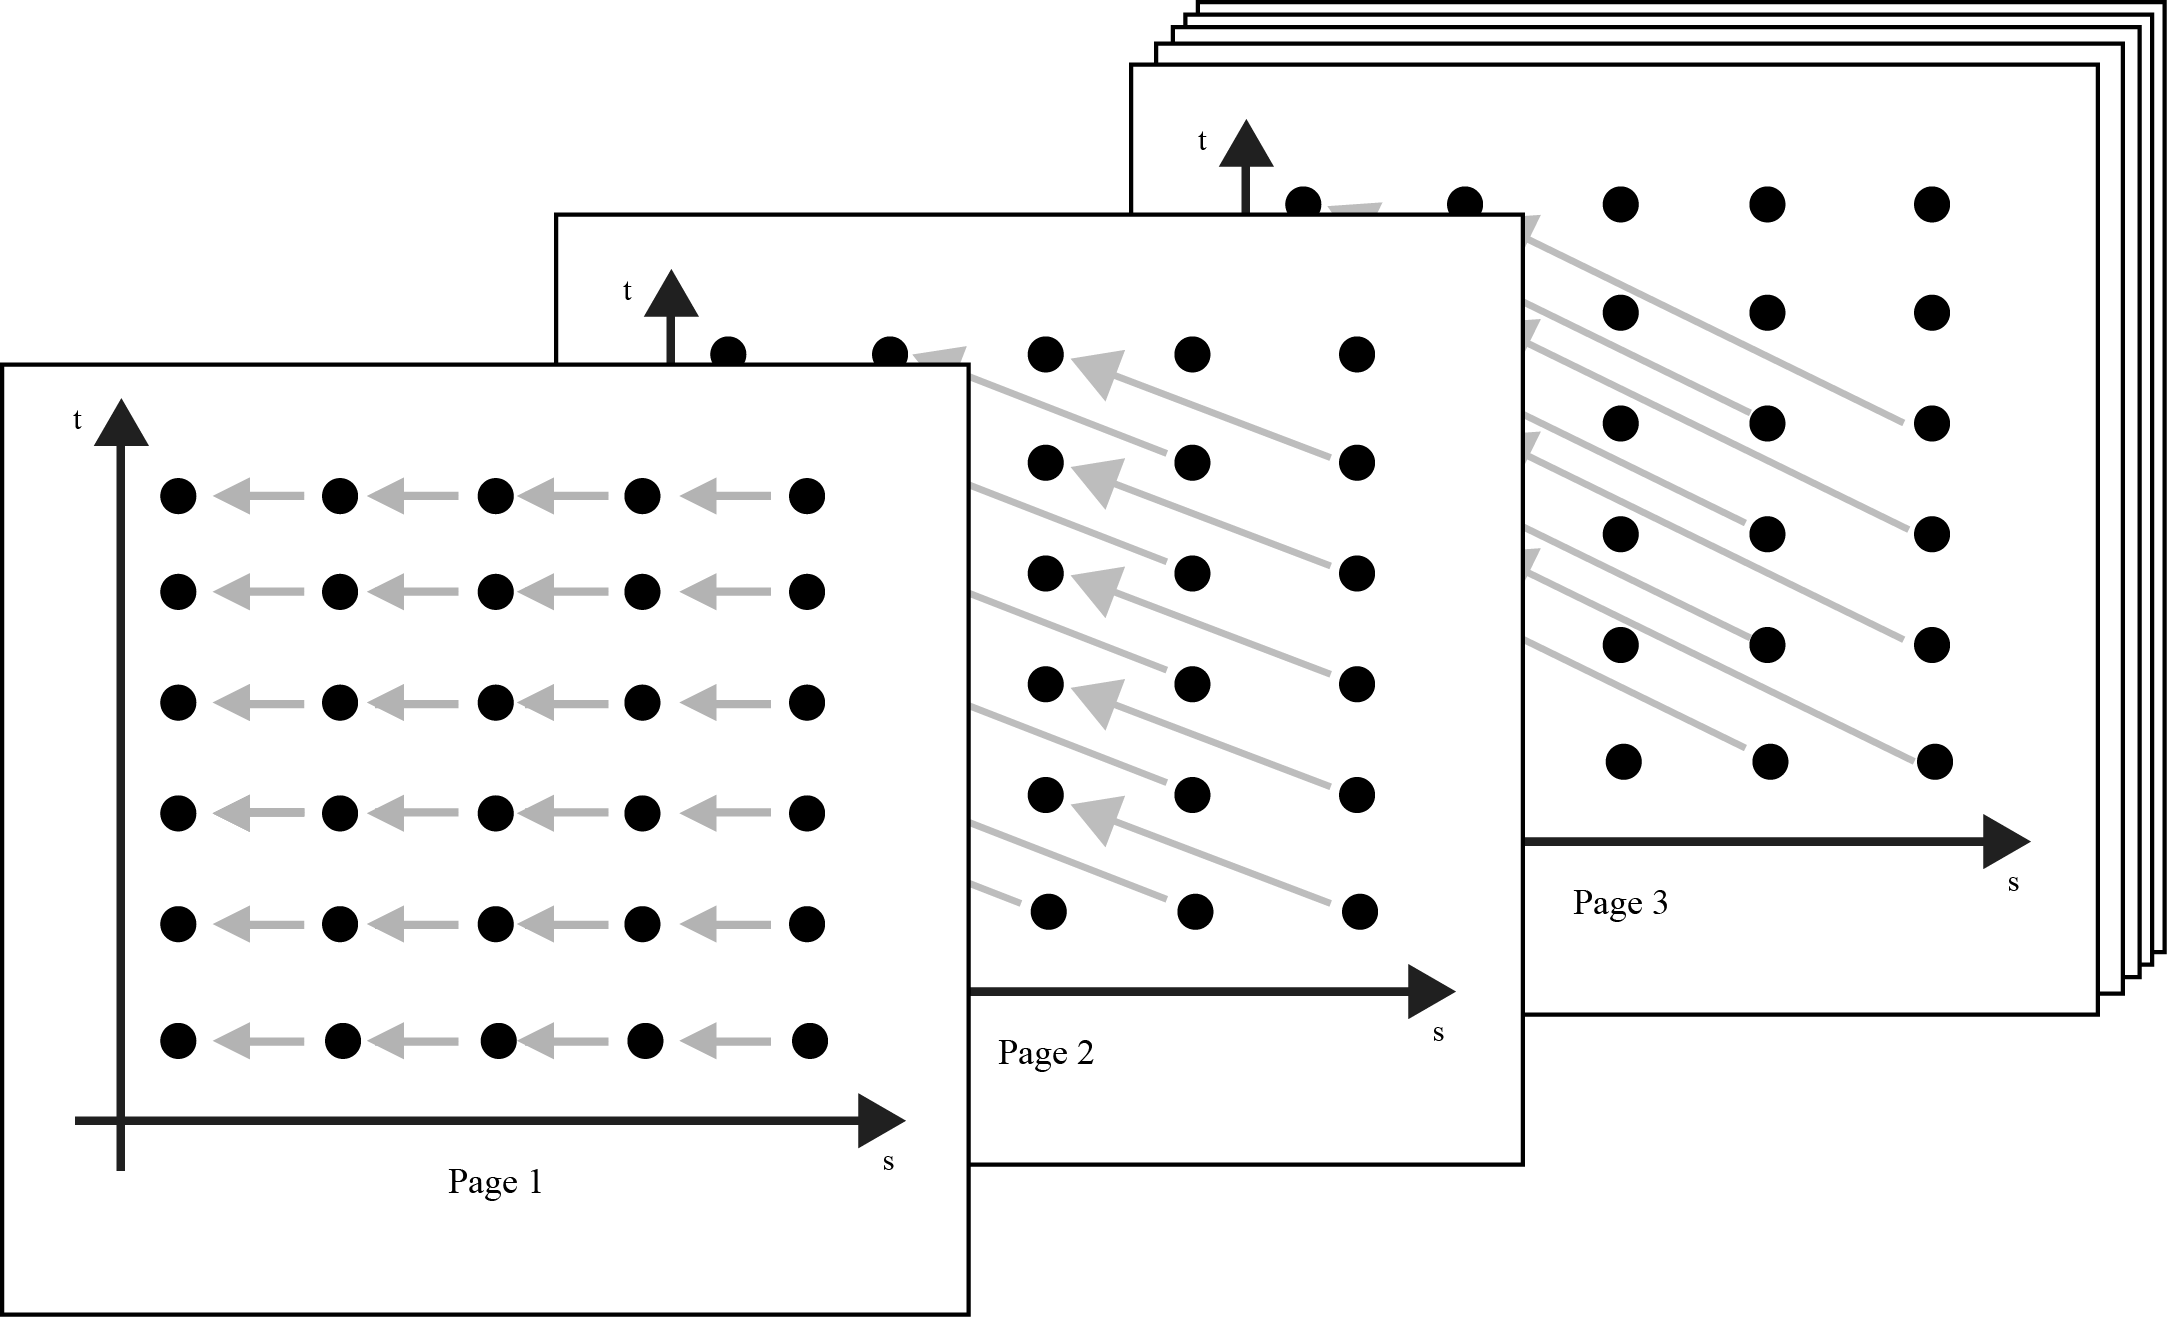
\includegraphics[width=\linewidth]{figures/cover.png}
       \begin{minipage}{.35\linewidth}
    \begin{flushleft}
      \vspace{2em}
      {\fontsize{6pt}{2pt} \textit{Notes: These are notes live-tex'd
from a graduate course in Algebraic Geometry taught by Philip Engel at
the University of Georgia in Fall 2020. As such, any errors or
inaccuracies are almost certainly my own. } } \\
    \end{flushleft}
    \end{minipage}
    \hfill
    \begin{minipage}{.65\linewidth}
    \end{minipage}
  }







\begin{document}

\date{}
\maketitle
\begin{flushleft}
\textbf{D. Zack Garza} \\
\textit{University of Georgia} \\
\textit{dzackgarza@gmail.com} \\
{\tiny \textit{Last updated:} 2020-10-20 }
\end{flushleft}


\newpage
\tableofcontents

\hypertarget{prologue}{%
\section*{Prologue}\label{prologue}}
\addcontentsline{toc}{section}{Prologue}

These are notes live-tex'd from a graduate course in Algebraic Geometry
taught by Philip Engel at the University of Georgia in Fall 2020. As
such, any errors or inaccuracies are almost certainly my own.

\medskip
\begin{flushright}
  D. Zack Garza, \today \\
  \currenttime
\end{flushright}

\hypertarget{references}{%
\subsection{References}\label{references}}

\begin{itemize}
\tightlist
\item
  Gathmann's Algebraic Geometry
  notes\autocite{gathmannAlgebraicGeometry}
  \url{https://www.mathematik.uni-kl.de/~gathmann/class/alggeom-2019/alggeom-2019.pdf}
\end{itemize}

\hypertarget{notation}{%
\subsection{Notation}\label{notation}}

\begin{align*}  
V(I) && \text{The variety associated to an ideal } I \normal \kx{n}
.\end{align*}

\newpage

\hypertarget{friday-august-21}{%
\section{Friday, August 21}\label{friday-august-21}}

\begin{quote}
Ref:

\url{https://www.mathematik.uni-kl.de/~gathmann/class/alggeom-2019/alggeom-2019.pdf}
\end{quote}

General idea: functions a coordinate ring \(R[x_1, \cdots, x_n]/I\) will
correspond to the geometry of the variety cut out by \(I\).\footnote{Example
  footnote.}

\begin{example}

\hfill

\begin{itemize}
\item
  \(x^2 + y^2 - 1\) defines a circle, say, over \(\RR\)
\item
  \(y^2 = x^3-x\) gives an elliptic curve:

  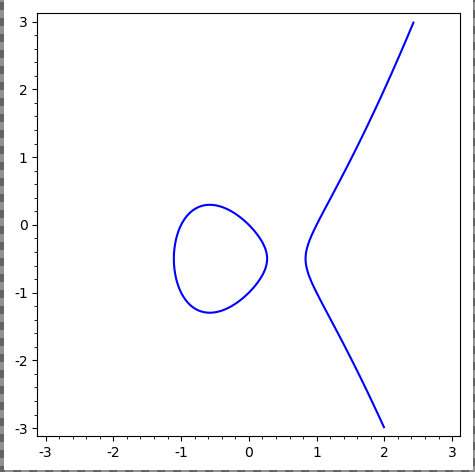
\includegraphics{figures/image_2020-08-21-01-04-22.png}
\item
  \(x^n+y^n-1\): does it even contain a \(\QQ\dash\)point? (Fermat's
  Last Theorem)
\item
  \(x^2 + 1\), which has no \(\RR\dash\)points.
\item
  \(x^2 + y^2 + 1/\RR\) vanishes nowhere, so its ring of functions is
  not \(\RR[x, y] / \gens{x^2 + y^2 + 1}\) (problem: \(\RR\) is not
  algebraically closed)
\item
  \(x^2 - y^2 = 0\) over \(\CC\) is not a manifold (no chart at the
  origin):

  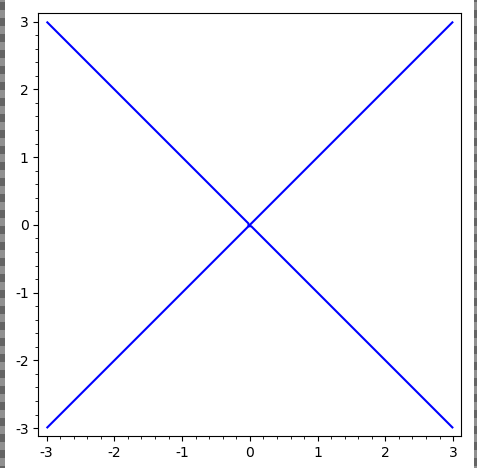
\includegraphics{figures/image_2020-08-21-01-23-32.png}
\item
  \(x+y+1/\FF_3\), which has 3 points over \(\FF_3^2\), but
  \(f(x, y) = (x^3 - x)(y^3-y)\) vanishes at every point

  \begin{itemize}
  \item
    Not possible when algebraically closed (is there nonzero polynomial
    that vanishes on every point in \(\CC\)?)
  \item
    \(V(f) = \FF_3^2\), so the coordinate ring is zero instead of
    \(\FF_3[x, y]/\gens{f}\) (addressed by scheme theory)
  \end{itemize}
\end{itemize}

\end{example}

\begin{theorem}[Harnack Curve Theorem]

If \(f \in \RR[x, y]\) is of degree \(d\), then
\begin{align*}  
\pi_1 V(f) \subseteq \RR^2 \leq 1 + {(d-1)(d-2) \over 2}
\end{align*}

\begin{quote}
Actual statement: the number of connected components is bounded above by
this quantity.
\end{quote}

\end{theorem}

\begin{example}

Take the curve
\begin{align*}  
X = \theset{(x, y, z) = (t^3, t^4, t^5) \in \CC^3 \suchthat t\in \CC}
.\end{align*}

Then \(X\) is cut out by three equations:

\begin{itemize}
\tightlist
\item
  \(y^2 = xz\)
\item
  \(x^2 = yz\)
\item
  \(z^2 = x^2 y\)
\end{itemize}

\end{example}

\begin{exercise}

Show that the vanishing locus of the first two equations above is
\(X\union L\) for \(L\) a line.

\end{exercise}

Compare to linear algebra: codimension \(d\) iff cut out by exactly
\(d\) equations.

\begin{example}

Given the Riemann surface
\begin{align*}  
y^2 = (x-1)(x-2)\cdots(x-2n)
,\end{align*} how to visualize the solution set?

Fact: on \(\CC\) with some slits, you can consistently choose a square
root of the RHS.

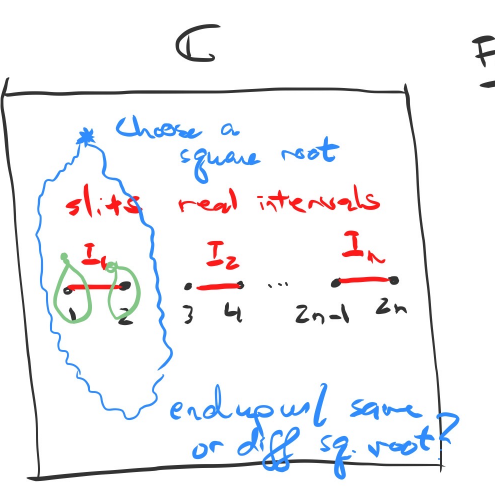
\includegraphics{figures/image_2020-08-21-01-31-47.png}

Away from \(x=1, \cdots, 2n\), there are two solutions for \(y\) given
\(x\).

After gluing along strips, obtain:

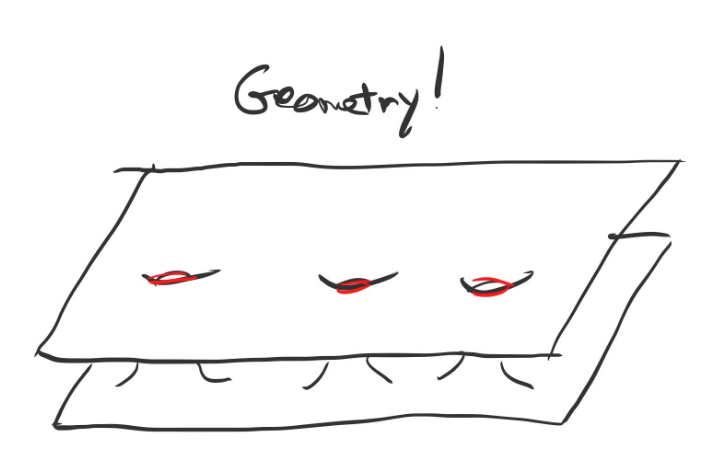
\includegraphics{figures/image_2020-08-21-01-32-48.png}

\end{example}

\hypertarget{tuesday-august-25}{%
\section{Tuesday, August 25}\label{tuesday-august-25}}

Let \(k = \bar k\) and \(R\) a ring containing ideals \(I, J\).

\begin{definition}[Radical]

Recall that the \emph{radical} of \(I\) is defined as
\begin{align*}  
\sqrt{I} = \ts{r\in R \st r^k\in I \text{ for some } k\in \NN}
.\end{align*}

\end{definition}

\begin{example}

Let \(I = (x_1, x_2^2) \subset \CC[x_1, x_2]\), so
\(I = \ts{ f_1 x_1 + f_2 x_2 \st f_1, f_2 \in \CC[x_1, x_2]}\). Then
\(\sqrt{I} = (x_1, x_2)\), since
\(x_2^2 \in I \implies x_2 \in \sqrt{I}\).

\end{example}

Given \(f\in k[x_1, \cdots, x_n]\), take its value at
\(a = (a_1, \cdots, a_n)\) and denote it \(f(a)\). Set \(\deg(f)\) to be
the largest value of \(i_1 + \cdots + i_n\) such that the coefficient of
\(\prod x_j ^{i_j}\) is nonzero.

\begin{example}

\(\deg(x_1 + x_2^2 + x_1 x_2^3 = 4)\)

\end{example}

\begin{definition}[Affine Variety]

\hfill

\begin{enumerate}
\def\labelenumi{\arabic{enumi}.}
\tightlist
\item
  Affine \(n\dash\)space \(\AA^n = \AA_k^n\) is defined as
  \(\theset{(a_1, \cdots, a_n) \suchthat a_i \in k}\).
\end{enumerate}

\begin{quote}
Remark: not \(k^n\), since we won't necessarily use the vector space
structure (e.g.~adding points).
\end{quote}

\begin{enumerate}
\def\labelenumi{\arabic{enumi}.}
\setcounter{enumi}{1}
\tightlist
\item
  Let \(S\subset k[x_1, \cdots, x_n]\) to be a set of polynomials. Then
  define \(V(S) = \ts{x\in \AA^n \st f(x) = 0} \subset \AA^n\) to be an
  \emph{affine variety}.
\end{enumerate}

\end{definition}

\begin{example}

\hfill

\begin{itemize}
\tightlist
\item
  \(\AA^n = V(0)\).
\item
  For any point \((a_1, \cdots, a_n)\in \AA^n\), then
  \(V(x_1 - a_1, \cdots, x_n - a_n) = \theset{a_1, \cdots, a_n}\)
  uniquely determines the point.
\item
  For any finite set \(r_1, \cdots, r_k \in \AA^1\), there exists a
  polynomial \(f(x)\) whose roots are \(r_i\).
\end{itemize}

\end{example}

\begin{remark}

We may as well assume \(S\) is an ideal by taking the ideal it
generates,
\(S\subseteq \gens{S} = \ts{\sum g_i f_i \suchthat g_i \in k[x_1, \cdots, x_n],\, f_i\in S}\).
Then \(V(\gens{S}) \subset V(S)\).

Conversely, if \(f_1, f_2\) vanish at \(x\in \AA^n\), then
\(f_1 + f_2, gf_1\) also vanish at \(x\) for all
\(g\in k[x_1, \cdots, x_n]\). Thus \(V(S) \subset V(\gens{S})\).

\end{remark}

\begin{proposition}[Properties and Definitions of Ideal Operations]

\hfill

\begin{itemize}
\tightlist
\item
  \(I+J \da \ts{f+g \st f\in I,\, g\in J}\).
\item
  \(IJ \da \ts{\sum_{i=1}^N f_i g_i \st f_i\in I,\, g_i\in J, N\in \NN}\).
\item
  If \(I+J = \gens{1}\) then \(I\intersect J = IJ\) (coprime or
  comaximal)
\end{itemize}

\end{proposition}

Note that if \(I = \gens{a}\) and \(J = \gens{b}\), then
\(I + J = \gens{a} + \gens{b} = \gens{a, b}\).

\begin{proposition}[Properties of $V$]

\hfill

\begin{enumerate}
\def\labelenumi{\arabic{enumi}.}
\tightlist
\item
  If \(S_1 \subseteq S_2\) then \(V(S_1) \supseteq V(S_2)\).
\item
  \(V(S_1) \union V(S_2) = V(S_1 S_2) = V(S_1 \intersect S_2)\).
\item
  \(\bigcap V(S_i) = V\qty{\bigcup S_i}\).
\end{enumerate}

\end{proposition}

We thus have a map
\begin{align*}  
V: \ts{\text{Ideals in } k[x_1, \cdots, x_n]} \to \ts{\text{Affine varieties in } \AA^n}
.\end{align*}

\begin{definition}[The Ideal of a Set]

Let \(X\subset \AA^n\) be any set, then \emph{the ideal of \(X\)} is
defined as
\begin{align*}  
I(X) \da\ts{f\in k[x_1, \cdots, x_n] \st f(x) = 0\, \forall x\in X}
.\end{align*}

\end{definition}

\begin{example}

Let \(X\) be the union of the \(x_1\) and \(x_2\) axes in \(\AA^2\),
then \(I(X) = (x_1 x_2) = \ts {x_1 x_2 g\st g\in k[x_1, x_2]}\).

\end{example}

Note that if \(X_1 \subset X_2\) then \(I(X_1) \subset I(X_2)\).

\begin{proposition}[The Image of $V$ is Radical]

\(I(X)\) is a radical ideal, i.e.~\(I(X) = \sqrt{I(X)}\).

This is because \(f(x)^k = 0 \forall x\in X\) implies \(f(x) = 0\) for
all \(x\in X\), so \(f^k \in I(X)\) and thus \(f\in I(X)\).

\end{proposition}

Our correspondence is thus
\begin{align*}  
\correspond{\text{Ideals in } k[x_1, \cdots, x_n]} &\mapsvia{V} \correspond{\text{Affine Varieties}} \\
\correspond{\text{Radical Ideals}} &\xleftarrow{I} \correspond{\text{?}}
.\end{align*}

\begin{proposition}[Hilbert Nullstellensatz (Zero Locus Theorem)]

\hfill

\begin{enumerate}
\def\labelenumi{\alph{enumi}.}
\item
  For any affine variety \(X\), \(V(I(X)) = X\).
\item
  For any ideal \(J \subset k[x_1, \cdots, x_n]\),
  \(I(V(J)) = \sqrt{J}\).
\end{enumerate}

\end{proposition}

Thus there is a bijection between radical ideals and affine varieties.

\hypertarget{proof-of-nullstellensatz}{%
\subsection{Proof of Nullstellensatz}\label{proof-of-nullstellensatz}}

\begin{remark}

Recall the Hilbert Basis Theorem: any ideal in a finitely generated
polynomial ring over a field is again finitely generated.

\end{remark}

We need to show 4 inclusions, 3 of which are easy.

a: \(X \subset V(I(X))\):

\begin{itemize}
\tightlist
\item
  If \(x\in X\) then \(f(x) = 0\) for all \(f\in I(X)\).
\item
  So \(x\in V(I(X))\), since every \(f\in I(X)\) vanishes at \(x\).
\end{itemize}

b: \(\sqrt{J} \subset I(V(J))\):

\begin{itemize}
\tightlist
\item
  If \(f\in \sqrt{J}\) then \(f^k \in J\) for some \(k\).
\item
  Then \(f^k(x) = 0\) for all \(x\in V(J)\).
\item
  So \(f(x) = 0\) for all \(x\in V(J)\).
\item
  Thus \(f\in I(V(J))\).
\end{itemize}

c: \(V(I(X)) \subset X\):

\begin{itemize}
\tightlist
\item
  Need to now use that \(X\) is an affine variety.

  \begin{itemize}
  \tightlist
  \item
    Counterexample: \(X = \ZZ^2 \subset \CC^2\), then \(I(X) = 0\). But
    \(V(I(X)) = \CC^2\), but \(\CC^2 \not\subset \ZZ^2\).
  \end{itemize}
\item
  By (b), \(I(V(J)) \supset \sqrt{J} \supset J\).
\item
  Since \(V(\wait)\) is order-reversing, taking \(V\) of both sides
  reverses the containment.
\item
  So \(V(I(V(J))) \subset V(J)\), i.e.~\(V(I(X)) \subset X\).
\end{itemize}

d: \(I(V(J)) \subset \sqrt{J}\) (hard direction)

\begin{theorem}[1st Version of Nullstellensatz]

Suppose \(k\) is algebraically closed and uncountable (still true in
countable case by a different proof).

Then the maximal ideals in \(k[x_1, \cdots, x_n]\) are of the form
\((x_1 - a_1, \cdots, x_n - a_n)\).

\end{theorem}

\begin{proof}

Let \(\mfm\) be a maximal ideal, then by the Hilbert Basis Theorem,
\(\mfm = \gens{f_1, \cdots, f_r}\) is finitely generated.

Let \(L = \QQ[\ts {c_i}]\) where the \(c_i\) are all of the coefficients
of the \(f_i\) if \(\ch(K) = 0\), \textbf{or} \(\FF_p[\ts {c_i}]\) if
\(\ch(k) = p\). Then \(L\subset k\).

Define \(\mfm_0 = \mfm\intersect L[x_1, \cdots, x_n]\). Note that by
construction, \(f_i \in \mfm_0\) for all \(i\), and we can write
\(\mfm = \mfm_0 \cdot k[x_1, \cdots, x_n]\).

\textbf{Claim}: \(\mfm_0\) is a maximal ideal.

If it were the case that
\begin{align*}  
\mfm_0 \subsetneq \mfm_0' \subsetneq L[x_1, \cdots, x_n]
,\end{align*} then
\begin{align*}  
\mfm_0\cdot k[x_1, \cdots, x_n] \subsetneq \mfm_0'\cdot k[x_1, \cdots, x_n]  \subsetneq k[x_1, \cdots, x_n]
.\end{align*}

\begin{quote}
So far: constructed a smaller polynomial ring and a maximal ideal in it.
\end{quote}

Thus \(L[x_1, \cdots, x_n]/\mfm_0\) is a field that is finitely
generated over either \(\QQ\) or \(\FF_p\).

\begin{theorem}[Noether Normalization]

Any finitely-generated field extension \(k_1 \injects k_2\) is a finite
extension of a purely transcendental extension, i.e.~there exist
\(t_1, \cdots, t_\ell\) such that \(k_2\) is finite over
\(k_1(t_1, \cdots, t_\ell)\).

\end{theorem}

\begin{quote}
Note: this theorem is perhaps more important than the Nullstellensatz!
\end{quote}

Thus \(L[x_1, \cdots, x_n]/\mfm_0\) is finite over some
\(\QQ(t_1, \cdots, t_n)\), and since \(k\) is uncountable, there exists
an embedding \(\QQ(t_1, \cdots, t_n) \injects k\).

\begin{quote}
Use the fact that there are only countably many polynomials over a
countable field.
\end{quote}

This extends to an embedding of
\(\phi: L[x_1, \cdots, x_n]/\mfm_0 \injects k\) since \(k\) is
algebraically closed. Letting \(a_i\) be the image of \(x_i\) under
\(\phi\), then \(f(a_1, \cdots, a_n) = 0\) by construction,
\(f_i \in (x_i - a_i)\) implies that \(\mfm = (x_i - a_i)\) by
maximality.

\end{proof}

\hypertarget{thursday-august-27}{%
\section{Thursday, August 27}\label{thursday-august-27}}

Recall Hilbert's Nullstellensatz:

\begin{enumerate}
\def\labelenumi{\alph{enumi}.}
\item
  For any affine variety, \(V(I(X)) = X\).
\item
  For any ideal \(J\normal k[x_1, \cdots, x_n]\),
  \(I(V(J)) = \sqrt{J}\).
\end{enumerate}

So there's an order-reversing bijection
\begin{align*}  
\correspond{\text{Radical ideals } k[x_1, \cdots, x_n]} \to{V(\wait)}{I(\wait)}
\correspond{\text{Affine varieties in } \AA^n}
.\end{align*}

In proving \(I(V(J)) \subseteq \sqrt{J}\), we had an important lemma
(Noether Normalization): the maximal ideals of \(k[x_1, \cdots, x_n]\)
are of the form \(\gens{x-a_1, \cdots, x-a_n}\).

\begin{corollary}[?]

If \(V(I)\) is empty, then \(I = \gens{1}\).

\begin{quote}
Slogan: the only ideals that vanish nowhere are trivial. No common
vanishing locus \(\implies\) trivial ideal, so there's a linear
combination that equals 1.
\end{quote}

\end{corollary}

\begin{proof}

By contrapositive, suppose \(I\neq \gens{1}\). By Zorn's Lemma, these
exists a maximal ideals \(\mfm\) such that \(I \subset \mfm\). By the
order-reversing property of \(V(\wait)\), \(V(\mfm) \subseteq V(I)\). By
the classification of maximal ideals,
\(\mfm = \gens{x-a_1, \cdots, x-a_n}\), so
\(V(\mfm) = \theset{a_1, \cdots, a_n}\) is nonempty.

\end{proof}

Returning to the proof that \(I(V(J)) \subseteq \sqrt{J}\): let
\(f\in V(I(J))\), we want to show \(f\in \sqrt{J}\). Consider the ideal
\(\tilde J \da J + \gens{ft - 1} \subseteq k[x_1, \cdots, x_n, t]\).

Observation: \(f = 0\) on all of \(V(J)\) by the definition of
\(I(V(J))\). But \(ft-1 \neq 0\) if \(f=0\), so
\(V(\tilde J) = V(G) \intersect V(ft-1) = \emptyset\).

\begin{figure}
\centering
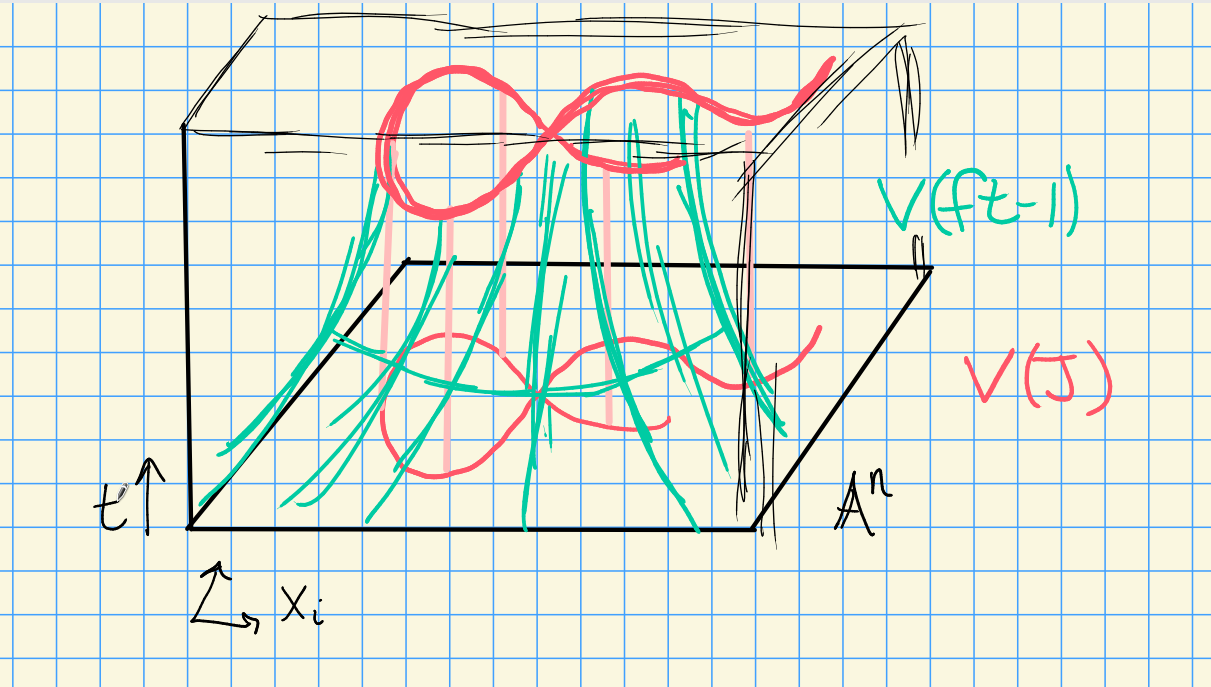
\includegraphics{figures/image_2020-08-27-09-56-33.png}
\caption{Effect, a hyperbolic tube around \(V(J)\), so both can't
vanish}
\end{figure}

Applying the corollary \(\tilde J = (1)\), so
\(1 = \gens{ft-1} g_0(x_1, \cdots, x_n, t) + \sum f_i g_i(x_1, \cdots, x_n, t)\)
with \(f_i \in J\). Let \(t^N\) be the largest power of \(t\) in any
\(g_i\). Thus for some polynomials \(G_i\), we have
\begin{align*}  
f^N \da (ft-1) G_0(x_1, \cdots, x_n, ft) + \sum f_i G_i(x_1, \cdots, x_n, ft)
\end{align*} noting that \(f\) does not depend on \(t\).

Now take \(k[x_1, \cdots, x_n, t]/\gens{ft-1}\), so \(ft=1\) in this
ring. This kills the first term above, yielding
\begin{align*}  
f^N = \sum f_i G_i(x_1, \cdots, x_n, 1) \in k[x_1, \cdots, x_n, t]/\gens{ft-1}
.\end{align*}

Observation: there is an inclusion
\begin{align*}  
k[x_1, \cdots, x_n] \injects
k[x_1, \cdots, x_n, t]/\gens{ft-1}
.\end{align*}

\begin{exercise}

Why is this true?

\end{exercise}

Since this is injective, this identity also holds in
\(k[x_1, \cdots, x_n]\). But \(f_i\in J\), so \(f\in \sqrt{I}\).

\begin{example}

Consider \(k[x]\). If \(J\subset k[x]\) is an ideal, it is principal, so
\(J = \gens{f}\). We can factor \(f(x) = \prod_{i=1}^k (x-a_i)^{n_i}\)
and \(V(f) = \ts{a_1, \cdots, a_k}\). Then
\(I(V(f)) = \gens{(x-a_1)(x-a_2)\cdots(x-a_k)} = \sqrt{J} \subsetneq J\).
Note that this loses information.

\end{example}

\begin{example}

Let \(J = \gens{x-a_1, \cdots, x-a_n}\), then \(I(V(J)) = \sqrt{J} = J\)
with \(J\) maximal. Thus there is a correspondence
\begin{align*}  
\correspond{\text{Points of } \AA^n} \iff 
\correspond{\text{Maximal ideals of }k[x_1, \cdots, x_n]}
.\end{align*}

\end{example}

\begin{theorem}[Properties of $I$]

\hfill

\begin{enumerate}
\def\labelenumi{\alph{enumi}.}
\item
  \(I(X_1 \union X_2) = I(X_1) \intersect I(X_2)\).
\item
  \(I(X_1) \intersect I(X_2) = \sqrt{I(X_1) + I(X_2)}\).
\end{enumerate}

\end{theorem}

\begin{proof}

We proved (a) on the variety side.

For (b), by the Nullstellensatz, \(X_i = V(I(X_i))\), so
\begin{align*}  
I(X_1\intersect X_2) 
&=
I\qty{ VI(X_1) \intersect VI(X_2)} \\
&=
IV\qty{I(X_1) + I(X_2)} \\
&= \sqrt{I(X_1) + I(X_2)}
.\end{align*}

\end{proof}

\begin{example}

Example of property (b):

Take \(X_1 = V(y-x^2)\) and \(X_2 = V(y)\), a parabola and the
\(x\dash\)axis.

\begin{figure}
\centering
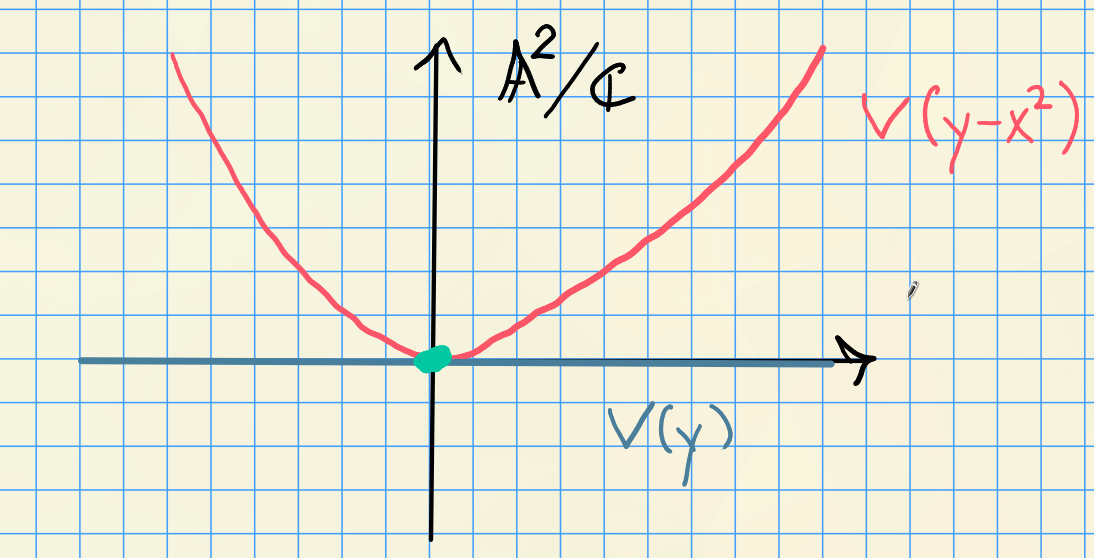
\includegraphics{figures/image_2020-08-27-10-26-45.png}
\caption{Image}
\end{figure}

Then \(X_1 \intersect X_2 = \ts{(0, 0)}\), and
\(I(X_1) + I(X_2) = \gens{y-x^2, y} = \gens{x^2, y}\), but
\(I(X_1 \intersect X_2) = \gens{x, y} = \sqrt{\gens{x^2, y}}\).

\end{example}

\begin{proposition}[?]

If \(f, g\in k[x_1, \cdots, x_n]\), and suppose \(f(x) = g(x)\) for all
\(x\in \AA^n\). Then \(f = g\).

\end{proposition}

\begin{proof}

Since \(f-g\) vanishes everywhere,
\(f-g \in I(\AA^n) = I(V(0)) = \sqrt{0} = 0\).

\end{proof}

More generally suppose \(f(x) = g(x)\) for all \(x\in X\), where \(X\)
is some affine variety. Then by definition, \(f-g \in I(X)\), so a
``natural'' space of functions on \(X\) is \(k[x_1,\cdots, x_n]/I(X)\).

\begin{definition}[Coordinate Ring]

For an affine variety \(X\), the \emph{coordinate ring of \(X\)} is
\begin{align*}  
A(X) \da k[x_1, \cdots, x_n]/ I(X)
.\end{align*}

Elements \(f\in A(X)\) are called \emph{polynomial} or \emph{regular}
functions on \(X\).

\end{definition}

Observation: The constructions \(V(\wait), I(\wait)\) work just as well
for \(A(X)\) and \(X\).

Given any \(S\subset A(Y)\) for \(Y\) an affine variety,
\begin{align*}  
V(S) = V_Y(S) \da\ts{x\in Y \st f(x) = 0\,\,\forall f\in S}
.\end{align*}

Given \(X\subset Y\) a subset,
\begin{align*}  
I(X) = I_Y(X) \da\ts{f\in A(Y) \st f(x) = 0\,\,\forall x\in X} \subseteq A(Y)
.\end{align*}

\begin{example}

For \(X\subset Y \subset \AA^n\), we have
\(I(X) \supset I(Y) \supset I(\AA^n)\), so we have maps

\begin{center}\includesvg[width=\linewidth]{2735152d58f437dbff3ae1ed22eebccf3c55c71b}\end{center}

\end{example}

\begin{theorem}[?]

Let \(X\subset Y\) be an affine subvariety, then

\begin{enumerate}
\def\labelenumi{\alph{enumi}.}
\item
  \(A(X) = A(Y) / I_Y(X)\)
\item
  There is a correspondence
  \begin{align*}  
  \correspond{\text{Affine subvarieties of }Y} 
  &\iff \correspond{\text{Radical ideals in }A(Y)} \\
  X &\mapsto I_Y(X) \\
  V_Y(J) &\mapsfrom J
  .\end{align*}
\end{enumerate}

\end{theorem}

\begin{proof}

Properties are inherited from the case of \(\AA^n\), see exercise in
Gathmann.

\end{proof}

\begin{example}

Let \(Y = V(y-x^2) \subset \AA^2/\CC\) and
\(X = \ts{(1, 1)} = V(x-1, y-1)\subset \AA^2/\CC\).

Then there is an inclusion \(\gens{y-x^2} \subset \gens{x-1, y-1}\)
(e.g.~by Taylor expanding about the point \((1, 1)\)), and there is a
map

\begin{center}\includesvg[width=\linewidth]{dbfa48c9f7c3b754eac5bfdcd6d2857857406650}\end{center}

\end{example}

\hypertarget{tuesday-september-01}{%
\section{Tuesday, September 01}\label{tuesday-september-01}}

Last time: \(V(I) = \ts{x\in \AA^n \st f(x) = 0 \, \forall x\in I}\) and
\(I(X) = \ts{f\in k[x_1, \cdots, x_n] \st f(x) = 0\, \forall x\in X}\).
We proved the Hilbert Nullstellensatz \(I(V(J)) = \sqrt{J}\), defined
the coordinate ring of an affine variety \(X\) as
\(A(X) \da k[x_1, \cdots, x_n] / I(X)\), the ring of ``regular''
(polynomial) functions on \(X\).

Recall that a \emph{topology} on \(X\) can be defined as a collection of
``closed'' subsets of \(X\) that are closed under arbitrary
intersections and finite unions. A subset \(Y\subset X\) inherits a
subspace topology with closed sets of the form \(Z\intersect Y\) for
\(Z\subset X\) closed.

\begin{definition}[Zariski Topology]

Let \(X\) be an affine variety. The closed sets are affine subvarieties
\(Y\subset X\).

\end{definition}

We have \(\emptyset, X\) closed, since

\begin{enumerate}
\def\labelenumi{\arabic{enumi}.}
\tightlist
\item
  \(V_X(1) = \emptyset\),
\item
  \(V_X(0) = X\)
\end{enumerate}

Closure under finite unions: Let \(V_X(I), V_X(J)\) be closed in \(X\)
with \(I, J \subset A(X)\) ideals. Then
\(V_X(IJ) = V_X(I) \union V_X(J)\).

Closure under intersections: We have
\(\bigcap_{i\in \sigma} V_X(J) = V_X\qty{ \sum_{i\in \sigma} J_i}\).

\begin{remark}

There are few closed sets, so this is a ``weak'' topology.

\end{remark}

\begin{example}

Compare the classical topology on \(\AA^1/\CC\) to the Zariski topology.

Consider the set \(A\da \ts{x\in \AA^1/\CC \st \norm{x} \leq 1}\), which
is closed in the classical topology.

But \(A\) is not closed in the Zariski topology, since the closed
subsets are finite sets or the whole space.

\begin{quote}
Here the topology is in fact the cofinite topology.
\end{quote}

\end{example}

\begin{example}

Let \(f: \AA^1/k\to \AA^1/k\) be any injective map. Then \(f\) is
necessarily continuous wrt the Zariski topology.

\end{example}

Thus the notion of continuity is too weak in this situation.

\begin{example}

Consider \(X\cross Y\) a product of affine varieties. Then there is a
product topology where open sets are of the form
\(\bigcup_{i=1}^n U_i \cross V_i\) with \(U_i, V_i\) open in \(X, Y\)
respectively.

This is the wrong topology! On \(\AA^1 \cross \AA^1 = \AA^2\), the
diagonal \(\Delta \da V(x-y)\) is closed in the Zariski topology on
\(\AA^2\) but not in the product topology.

\end{example}

\begin{example}

Consider \(\AA^2/\CC\), so the closed sets are curves and points.
Observation: \(V(x_1 x_2 ) \subset \AA^2/\CC\) decomposed into the union
of the coordinate axes \(X_1 \da V(x_1)\) and \(X_2 \da V(x_2)\). The
Zariski topology can detect these decompositions.

\end{example}

\begin{definition}[Irreducibility and Connectedness]

Let \(X\) be a topological space.

\begin{enumerate}
\def\labelenumi{\alph{enumi}.}
\item
  \(X\) is \emph{reducible} iff there exist nonempty proper closed
  subsets \(X_1 ,X_2 \subset X\) such that \(X = X_1 \union X_2\).
  Otherwise, \(X\) is said to be \emph{irreducible}.
\item
  \(X\) is \emph{disconnected} if there exist \(X_1, X_2 \subset X\)
  such that \(X = X_1 \disjoint X_2\). Otherwise, \(X\) is said to be
  \emph{connected}.
\end{enumerate}

\end{definition}

\begin{example}

\(V(x_1 x_2)\) is reducible but connected.

\end{example}

\begin{remark}

\(\AA^1/\CC\) is \emph{not} irreducible, since we can write
\(\AA^1/\CC = \ts{\norm{x} \leq 1} \union \ts{\norm{x} \geq 1}\).

\end{remark}

\begin{proposition}[?]

Let \(X\) be a disconnected affine variety with
\(X = X_1 \disjoint X_2\). Then \(A(X) \cong A(X_1) \cross A(X_2)\).

\end{proposition}

\begin{proof}

We have \(X_1 \union X_2 = X\), so
\(I(X_1) \intersect I(X_2) = I(X) = (0)\) in the coordinate ring
\(A(X)\) (recalling that it is a quotient by \(I(X)\).)

Since \(X_1 \intersect X_1 \emptyset\), we have
\begin{align*}  
I(X_1 \intersect X_2) = \sqrt{I(X_1) + I(X_2) } = I(\emptyset) = \gens{1}
.\end{align*}

Thus \(I(X_1) + I(X_2) = \gens{1}\), and by the Chinese Remainder
Theorem, the following map is an isomorphism:
\begin{align*}  
A(X) \to A(X)/I(X_1) \cross A(X) / I(X_2)
.\end{align*}

But the codomain is precisely \(A(X_1) \cross A(X_2)\).

\end{proof}

\begin{proposition}[?]

An affine variety \(X\) is irreducible \(\iff\) \(A(X)\) is an integral
domain.

\end{proposition}

\begin{proof}

\(\implies\): By contrapositive, suppose \(f_1, f_2 \in A(X)\) are
nonzero with \(f_1 f_2 = 0\). Let \(X_i = V(f_i)\), then
\(X= V(0) = V(f_1 f_2) = X_1 \union X_2\) which are closed and proper
since \(f_i \neq 0\).

\hfill\break

\(\impliedby\): Suppose \(X\) is reducible with \(X = X_1 \union X_2\)
with \(X_i\) proper and closed. Define \(J_i \da I(X_i)\), and note
\(J_i \neq 0\) because \(V(J_i) = V(I(X_i)) = X_i\) by part (a) of the
Nullstellensatz.

So there exists a nonzero \(f_i \in J_i = I(X_i)\), so \(f_i\) vanishes
on \(X_i\). But then
\(V(f_1) \union V(f_2) \supset X_1 \union X_2 = X\), so
\(X= V(f_1 f_2)\) and \(f_1 f_2 \in I(X) = \gens{0}\) and
\(f_1 f_2 = 0\). So \(A(X)\) is not a domain.

\end{proof}

\begin{example}

Let \(X = \ts{p_1, \cdots, p_d}\) be a finite set in \(\AA^n\). The
Zariski topology on \(X\) is the discrete topology, and
\(X = \disjoint \ts{p_i}\). So
\begin{align*}  
A(X) = A(\disjoint \ts{p_i}) = \prod_{i=1}^d A({\ts{p_i}}) = \prod_{i=1}^d k[x_1, \cdots, x_n] / \gens{x_j - a_j(p_i)}_{j=1}^d
.\end{align*}

\end{example}

\begin{example}

Set \(V(x_1 x_2) = X\), then \(A(X) = k[x_1, x_2]/ \gens{x_1 x_2}\).
This not being a domain (since \(x_1 x_2 = 0\)) corresponds to
\(X = V(x_1) \union V(x_2)\) not being irreducible.

\end{example}

\begin{example}

\(\AA^2/k\) is irreducible since \(k[x_1, \cdots x_n]\) is a domain.

\end{example}

\begin{example}

Let \(X_1\) be the \(xy\) plane and \(X_2\) be the line parallel to the
\(y\dash\)axis through \(\thevector{0,0,1}\), and let
\(X= X_1 \disjoint X_2\). Then \(X_1 = V(z)\) and \(X_2 = V(x, z-1)\),
and \(I(X) = \gens{z} \cdots \gens{x, z-1}= \gens{xz, z^2 - z}\).

Then the coordinate ring is given by
\(A(X) = \CC[x, y, z] / \gens{xz, z^2 - z} = \CC[x, y, z] / \gens{z} \oplus \CC[x, y,z] / \gens{x, z-1}\).

\begin{figure}
\centering
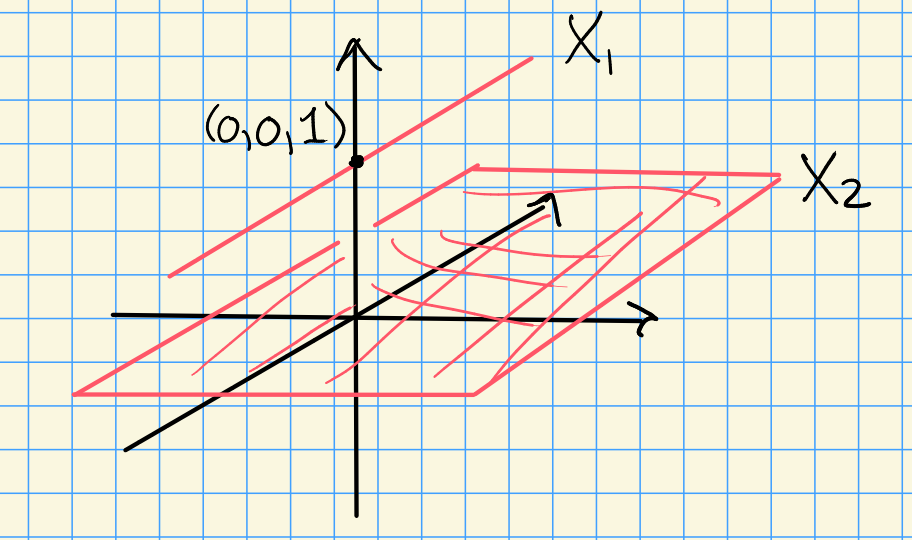
\includegraphics{figures/image_2020-09-01-10-43-00.png}
\caption{Image}
\end{figure}

\end{example}

\hypertarget{thursday-september-03}{%
\section{Thursday, September 03}\label{thursday-september-03}}

Recall that the Zariski topology is defined on an affine variety
\(X = V(J)\) with \(J \normal k[x_1, \cdots, x_n]\) by describing the
closed sets.

\begin{proposition}[?]

\(X\) is irreducible if its coordinate ring \(A(X)\) is a domain.

\end{proposition}

\begin{proposition}[?]

There is a 1-to-1 correspondence
\begin{align*}  
\correspond{\text{Irreducible subvarieties} \\ \text{of }X}
\iff
\correspond{\text{Prime ideals} \\ \text{in }A(X)}
.\end{align*}

\end{proposition}

\begin{proof}

Suppose \(Y\subset X\) is an affine subvariety. Then
\begin{align*}  
A(X) / I_X(Y) = A(Y)
.\end{align*}

By NSS, there is a bijection between subvarieties of \(X\) and radical
ideals of \(A(X)\) where \(Y\mapsto I_X(Y)\). A quotient is a domain iff
quotienting by a prime ideal, so \(A(Y)\) is a domain iff \(I_X(Y)\) is
prime.

\end{proof}

Recall that \(\mfp \normal R\) is prime when
\(fg\in \mfp \iff f\in \mfp\) or \(g\in \mfp\). Thus
\(\bar f \bar g = 0\) in \(R/\mfp\) implies \(\bar f = 0\) or
\(\bar g = 0\) in \(R/\mfp\), i.e.~\(R/\mfp\) is a domain.

Finally note that prime ideals are radical (easy proof).

\begin{example}

Consider \(\AA^2/\CC\) and some subvarieties \(C_i\):

\begin{figure}
\centering
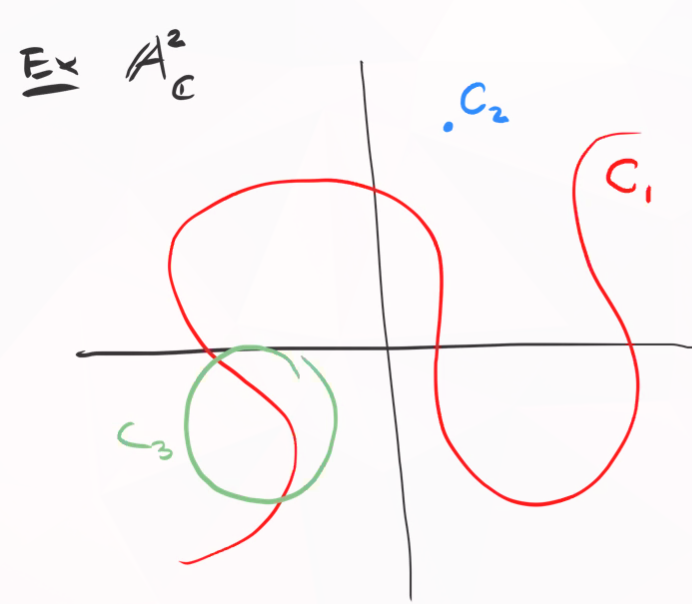
\includegraphics{figures/image_2020-09-03-09-47-09.png}
\caption{Subvarieties}
\end{figure}

Then irreducible subvarieties correspond to prime ideals in
\(\CC[x, y]\). Here \(C_1, C_3\) correspond to \(V(f), V(g)\) for
\(f,g\) irreducible polynomials, whereas \(C_2\) corresponds to a
maximal ideal, i.e.~\(V(x_1 - a_1, x_2 - a_2)\).

Note that \(I(C_1 \union C_2 \union C_3)\) is not a prime ideal, since
the variety is reducible as the union of 3 closed subsets.

\end{example}

\begin{example}

A finite set is irreducible iff it contains only one point.

\end{example}

\begin{example}

Any irreducible topological space is connected, since irreducible
requires a union but connectedness requires a \emph{disjoint} union.

\end{example}

\begin{example}

\(\AA^n/k\) is irreducible: by prop 2.8, its irreducible iff the
coordinate ring is a domain. However \(A(\AA^n) = k[x_1, \cdots, x_n]\),
which is a domain.

\end{example}

\begin{example}

\(V(x_1 x_2)\) is not irreducible, since it's equal to
\(V(x_1) \union V(x_2)\).

\end{example}

\begin{definition}[Noetherian Space]

A \emph{Noetherian} topological space \(X\) is a space with no infinite
strictly decreasing sequence of closed subsets.

\end{definition}

\begin{proposition}[?]

An affine variety \(X\) with the zariski topology is a noetherian space.

\end{proposition}

\begin{proof}

Let \(X_0 \supsetneq X_1 \supsetneq \cdots\) be a decreasing sequence of
closed subspaces. Then \(I(X_0) \subsetneq I(X_1) \subsetneq\). Note
that these containments are strict, otherwise we could use
\(V(I(X_1)) = X_1\) to get an equality in the original chain.

Recall that a ring \(R\) is Noetherian iff every ascending chain of
ideals terminates. Thus it suffices to show that \(A(X)\) is Noetherian.

We have \(A(X) = \kx{n} / I(X)\), and if this had an infinite chain
\(I_1 \subsetneq I_2 \subsetneq \cdots\) lifts to a chain in \(\kx{n}\),
which is Noetherian. A useful fact: \(R\) noetherian implies that
\(R[x]\) is noetherian, and fields are always noetherian.

\end{proof}

\begin{remark}

Any subspace \(A\subset X\) of a noetherian space is noetherian. To see
why, suppose we have a chain of closed sets in the subspace topology,
\begin{align*}  
A\intersect X_0 \supsetneq A\intersect X_1 \supsetneq \cdots
.\end{align*}

Then \(X_0 \supsetneq X_1 \supsetneq \cdots\) is a strictly decreasing
chain of closed sets in \(X\). Why strictly decreasing:
\(\intersect^n X_i = \intersect^{n+1} X_i \implies A\intersect^n X_i = A\intersect^{n+1} X_i\),
a contradiction.

\end{remark}

\begin{proposition}[Important]

Every noetherian space \(X\) is a finite union of irreducible closed
subsets, i.e.~\(X = \Union_{i=1}^k X_i\). If we further assume
\(X_i \not\subset X_j\) for all \(i, j\), then the \(X_i\) are unique up
to permutation.

\end{proposition}

\begin{remark}

The \(X_i\) are the \textbf{components} of \(X\). In the previous
example \(C_1 \union C_2 \union C_3\) has three components.

\end{remark}

\begin{proof}

If \(X\) is irreducible, then \(X=X\) and this holds.

Otherwise, write \(X = X_1 \union X_2\) with \(X_i\) proper closed
subsets. If \(X_1\) and \(X_1'\) are irreducible, we're done, so
otherwise suppose wlog \(X_1'\) is not irreducible.

Then we can express \(X = X_1 \union \qty{X_2 \union X_2'}\) with
\(X_2, X_2' \subset X_1'\) closed and proper.

Thus we can obtain a tree whose leaves are proper closed subsets:

\begin{figure}
\centering
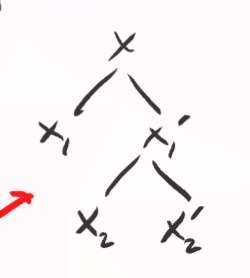
\includegraphics{figures/image_2020-09-03-10-15-53.png}
\caption{Image}
\end{figure}

This tree terminates because \(X\) is Noetherian: if it did not, this
would generate an infinite decreasing chain of subspaces.

We now want to show that the decomposition is unique if no two
components are contained in the other.

Suppose
\begin{align*}  
X= \Union_{i=1}^k X_i = \Union_{j=1}^\ell X_j'
.\end{align*}

Note that \(X_i \subset X\) implies that
\(X_i = \Union_{j=1}^\ell X_i \intersect X_j'\). But \(X_i\) is
irreducible and this would express \(X_i\) as a union of proper closed
subsets, so some \(X_i \intersect X_j'\) is \emph{not} a proper closed
subset.

Thus \(X_i = X_i \intersect X_j'\) for some \(j\), which forces
\(X_i \subset X_j'\). Applying the same argument to \(X_j'\) to obtain
\(X_j' \subset X_k\) for some \(k\).

Then \(X_i \subset X_j' \subset X_k\), but \(X_ i \not\subset X_j\) when
\(j\neq i\). Thus \(X_i = X_j' = X_k\), forcing the \(X_i\) to be unique
up to permutation.

\end{proof}

Recall from ring theory: for \(I\subset R\) and \(R\) noetherian, \(I\)
has a \emph{primary decomposition} \(I = \Intersect_{i=1}^k Q_i\) with
\(\sqrt{Q_i}\) prime. Assuming the \(Q_i\) are minimal in the sense that
\(\sqrt{Q_i} \not\subset \sqrt{Q_j}\) for any \(i, j\), this
decomposition is unique.

Applying this to \(I(X) \normal \kx{n} = R\) yields
\begin{align*}  
I(X) = \Intersect_{i=1}^k Q_i 
\implies
X  = V(I(X)) = \Union_{i=1}^k V(Q_i)
.\end{align*}

Letting \(P_i = \sqrt{Q_i}\), noting that the \(P_i\) are prime and thus
radical, we have \(V(Q_i) = V(P_i)\). Writing \(X = \Union V(P_i)\), we
have \(I(V(P_i)) = P_i\) and thus \(A(V(P_i)) = R/P_i\) is a domain,
meaning \(V(P_i)\) are irreducible affine varieties.

Conversely, if we express \(X = \Union X_i\), we have
\(I = I\qty{\Union X_i} = \Intersect I(X_i) = \Intersect P_i\) which are
irreducible since they are prime.

\begin{remark}

There is a correspondence
\begin{align*}  
\correspond{\text{Irreducible components} \\ \text{of } X} 
\iff
\correspond{\text{Minimal prime ideals} \\ \text{in } A(X)}
,\end{align*} where here \emph{minimal} is the condition that no pair of
ideals satisfies a subset containment.

\end{remark}

\begin{remark}

Let \(X\) be an irreducible topological space.

\begin{proposition}[1]

The intersection of nonempty two open sets is \emph{never} empty.

\end{proposition}

\begin{proof}

Let \(U, U'\) be open and \(X\setminus U, X\sm U'\) closed. Then
\(U\intersect U' = \emptyset \iff (X\sm U) \union (X\sm U') = X\), but
this is not possible since \(X\) is irreducible.

\end{proof}

\begin{quote}
Irreducible iff any two nonempty open sets intersect.
\end{quote}

\begin{proposition}[?]

Any nonempty open set is dense, i.e.~if \(U\subset X\) is open then its
closure \(\cl_X(U)\) is dense in \(X\).

\end{proposition}

\begin{proof}

Write \(X = \cl_X(U) \union (X\sm U)\). Since \(X\sm U \neq X\) and
\(X\) is irreducible, we have \(\cl_X(U) = X\).

\end{proof}

\end{remark}

\hypertarget{tuesday-september-08}{%
\section{Tuesday, September 08}\label{tuesday-september-08}}

Review: we discussed irreducible components. Recall that the
\emph{Zariski topology} on an affine variety \(X\) has affine
subvarieties as closed sets, and a \emph{noetherian space} has no
infinitely decreasing chains of closed subspaces.

We showed that any noetherian space has a decomposition into irreducible
components \(X = \union X_i\) with \(X_i\) closed, irreducible, and
unique such that no two are subsets of each other. Applying this to
affine varieties, a descending chain of subspaces
\(X_0 \supsetneq X_1 \cdots\) in \(X\) corresponds to an increasing
chain of ideals \(I(X_0) \subsetneq I(X_1) \cdots\) in \(A(X)\). Since
\(\kx{n}\) is a noetherian ring, this chain terminates, so affine
varieties are noetherian.

\hypertarget{dimension}{%
\subsection{Dimension}\label{dimension}}

\begin{definition}[Dimensions]

Let \(X\) be a topological space.

\begin{enumerate}
\def\labelenumi{\arabic{enumi}.}
\item
  The \emph{dimension} \(\dim X \in \NN\union\ts{\infty}\) is either
  \(\infty\) or the length \(n\) of the longest chain of
  \textbf{irreducible} closed subsets
  \(\emptyset \neq Y_0 \subsetneq \cdots \subsetneq Y_n \subset X\)
  where \(Y_n\) need not be equal to \(X\).
\item
  The \emph{codimension} of \(Y\) in \(X\), \(\codim_X(Y)\), for an
  irreducible subset \(Y\subseteq X\) is the length of the longest chain
  \(Y\subset Y_0 \subsetneq Y_1 \cdots \subset X\).
\end{enumerate}

\end{definition}

\begin{example}

Consider \(\AA^1/k\), what are the closed subsets? The finite sets, the
empty set, and the entire space.

What are the irreducible closed subsets? Every point is a closed subset,
so sets with more than one point are reducible. So the only irreducible
closed subsets are \(\ts{a}, \AA^1/k\), since an affine variety is
irreducible iff its coordinate ring is a domain and
\(A(\AA^1/k) = k[x]\). We can check
\begin{align*}  
\emptyset \subseteq Y_0 = \ts{a} \subseteq Y_1 = \AA^1/k
,\end{align*}

which is of length \(1\), so \(\dim(\AA^1/k) = 1\).

\begin{quote}
Note that we count the number of nontrivial strict subset containments
in this chain.
\end{quote}

\end{example}

\begin{example}

Consider \(V(x_1 x_2) \subset \AA^2/k\), the union of the \(x_i\) axes.
Then the closed subsets are \(V(x_1), V(x_2)\), along with finite sets
and their unions. What is the longest chain of irreducible closed
subsets?

Note that \(k[x_1, x_2] / \gens{x_1} \cong k[x_2]\) is a domain, so
\(V(x_i)\) are irreducible. So we can have a chain
\begin{align*}  
\emptyset \subsetneq \ts{a} \subsetneq V(x_1) \subset X
,\end{align*} where \(a\) is any point on the \(x_2\dash\)axis, so
\(\dim(X) = 1\).

The only closed sets containing \(V(x_1)\) are \(V(x_1)\union S\) for
\(S\) some finite set, which can not be irreducible.

\end{example}

\begin{remark}

You may be tempted to think that if \(X\) is noetherian then the
dimension is finite. However, finite dimension requires a bounded length
on descending/ascending chains, whereas noetherian only requires
``termination'', which may not happen in a bounded number of steps. So
this is \textbf{false}!

\end{remark}

\begin{example}

Take \(X = \NN\) and define a topology by setting closed subsets be the
sets \(\ts{0, \cdots, n}\) as \(n\) ranges over \(\NN\), along with
\(\NN\) itself. Is \(X\) noetherian? Check descending chains of closed
sets:

\begin{align*}  
\NN \supsetneq \ts{0, \cdots, N} \supsetneq \ts{0, \cdots, N-1} \cdots
,\end{align*}

which has length at most \(N\), so it terminates and \(X\) is
noetherian.

But note that all of these closed subsets \(X_N \da \ts{0, \cdots, N}\)
are irreducible. Why? If \(X_n = X_i \union X_j\) then one of \(i, j\)
is equal to \(N\), i.e \(X_i, X_j = X_N\).

So for every \(N\), there exists a chain of irreducible closed subsets
of length \(N\), implying that \(\dim(\NN) = \infty\).

\end{example}

\begin{remark}

Let \(X\) be an affine variety. There is a correspondence
\begin{align*}  
\correspond{\text{Chains of irreducible closed subsets} \\ Y_0 \subsetneq \cdots \subsetneq Y_n \text{ in } X}
\correspond{\text{Chains of prime ideals} \\ P_0\supsetneq \cdots \supsetneq P_n \text{ in } A(X)}
.\end{align*} Why? We have a correspondence between closed subsets and
radical ideals. If we specialize to irreducible, we saw that these
correspond to radical ideals \(I\subset A(X)\) such that
\(A(Y) \da A(X) / I\) is a domain, which precisely correspond to prime
ideal in \(A(X)\).

\end{remark}

We thus make the following definition:

\begin{definition}[Krull Dimension]

The \emph{krull dimension} of a ring \(R\) is the length \(n\) of the
longest chain of prime ideals
\begin{align*}  
P_0 \supsetneq P_1 \supsetneq \cdots \supsetneq P_n
.\end{align*}

\end{definition}

\begin{remark}

This uses the key fact from commutative algebra: a finitely generated
\(k\dash\)algebra \(M\) satisfies

\begin{enumerate}
\def\labelenumi{\arabic{enumi}.}
\tightlist
\item
  \(M\) has finite \(k\dash\)dimension
\item
  If \(M\) is a domain, every maximal chain has the same length.
\end{enumerate}

\end{remark}

\begin{remark}

From scheme theory: for any ring \(R\), there is an associated
topological space \(\spec R\) given by the set of prime ideals in \(R\),
where the closed sets are given by
\begin{align*}  
V(I) = \ts{\text{Prime ideals } \mfp \normal R \st I\subseteq \mfp }
.\end{align*}

If \(R\) is a noetherian ring, then \(\spec(R)\) is a noetherian space.

\end{remark}

\begin{example}

Using the fact above, let's compute \(\dim \AA^n/k\). We can take the
following chain of prime ideals in \(\kx{n}\):
\begin{align*}  
0 \subsetneq \gens{x_1} \subsetneq \gens{x_1, x_2} \cdots \subsetneq \gens{x_1, \cdots, x_n}
.\end{align*}

By applying \(V(\wait)\) we obtain
\begin{align*}  
\AA^n/k \supsetneq \AA^{n-1}/k \cdots \supsetneq \AA^0/k = \ts{0} \supsetneq \emptyset
,\end{align*} where we know each is irreducible and closed, and it's
easy to check that these are maximal:

If there were an ideal
\(\gens{x_1, x_2} \subset P \subset \gens{x_1, x_2, x_3}\), then take
\(P\intersect k[x_1, x_2, x_3] / \gens{x_1, x_2}\) which would yield a
polynomial ring in \(k[x_1]\). But we know the only irreducible sets in
\(\AA^1/k\) are a point and the entire space.

So this is a chain of maximal length, implying \(\dim \AA^n/k = n\).

\end{example}

\hypertarget{thursday-september-10}{%
\section{Thursday, September 10}\label{thursday-september-10}}

Recall that the dimension of a ring \(R\) is the length of the longest
chain of prime ideals. Similarly, for an affine variety \(X\), we
defined \(\dim X\) to be the length of the longest chain of irreducible
closed subsets.

These notions of dimension of the same when taking \(R = A(X)\),
i.e.~\(\dim \AA^n/k = n\).

\begin{proposition}[Dimensions]

Let \(k = \bar k\).

\begin{enumerate}
\def\labelenumi{\alph{enumi}.}
\tightlist
\item
  The dimension of \(k[x_1, \cdots, x_n]\) is \(n\).
\item
  All maximal chains of prime ideals have length \(n\).
\end{enumerate}

\end{proposition}

\hypertarget{proof-of-dimension-proposition}{%
\subsection{Proof of Dimension
Proposition}\label{proof-of-dimension-proposition}}

The case for \(n=0\) is trivial, just take \(P_0 = \gens{0}\). For
\(n=1\), easy to see since the only prime ideals in \(k[x]\) are
\(\gens{0}\) and \(\gens{x-a}\), since any polynomial factors into
linear factors.\\

Let \(P_0 \subsetneq \cdots \subsetneq P_m\) be a maximal chain of prime
ideals in \(\kx{n}\); we then want to show that \(m=n\). Assume
\(P_0 = \gens{0}\), since we can always extend our chain to make this
true (using maximality). Then \(P_1\) is a minimal prime and \(P_m\) is
a maximal ideal (and maximals are prime).

\begin{claim}

\(P_1\) is principle, i.e.~\(P_1 = \gens{f}\) for some irreducible
\(f\).

\end{claim}

\hypertarget{proof-that-p_1-is-principle}{%
\subsubsection{\texorpdfstring{Proof That \(P_1\) is
Principle}{Proof That P\_1 is Principle}}\label{proof-that-p_1-is-principle}}

\begin{claim}

\(\kx{n}\) is a unique factorization domain. This follows since \(k\) is
a UFD since it's a field, and \(R\) a UFD \(\implies R[x]\) is a UFD for
any \(R\).

\begin{quote}
See Gauss' lemma.
\end{quote}

\end{claim}

\begin{claim}

In a UFD, minimal primes are principal. Let \(r \in P\), and write
\(r = u \prod p_i^{n_i}\) with \(p_i\) irreducible and \(u\) a unit. So
some \(p_i\in P\), and \(p_i\) irreducible implies \(\gens{p_i}\) is
prime. Since \(0 \subsetneq \gens{p_i} \subset P\), but \(P\) was prime
and assumed minimal, so \(\gens{p_i} = P\).

\end{claim}

The idea is to now transfer the chain
\(P_0 \subsetneq \cdots \subsetneq P_m\) to a maximal chain in
\(k[x_1, \cdots, x_{n-1}]\). The first step is to make a linear change
of coordinates so that \(f\) is monic in the variable \(x_n\).

\begin{example}

Take \(f=x_1x_2 + x_3^2 x_4\) and map \(x_3 \mapsto x_3 + x_4\).

\end{example}

So write
\begin{align*}  
f(x_1, \cdots, x_n) = x_n^d + f_1(x_1, \cdots, x_{n-1}) x_n^{d-1} + \cdots + f_d(x_1, \cdots, x_{n-1})
.\end{align*}

We can then descend to \(\kx{n}\) to \(\kx{n}/\gens{f}\):

\begin{center}\includesvg[width=\linewidth]{cb63d23adbd3c993b1f5e3da6b1a70365137a7b2}\end{center}

The first set of downward arrows denote taking the quotient, and the
upward is taking inverse images, and this preserves strict inequalities.

\begin{definition}[Integral Extension]

An \emph{integral} ring extension \(R\injects R'\) of \(R\) is one such
that all \(r' \in R'\) satisfying a monic polynomial with coefficients
in \(R\), where \(R'\) is finitely generated.

\begin{quote}
In this case, also implies that \(R'\) is a finitely-generated \(R\)
module.
\end{quote}

\end{definition}

In this case, \(\kx{n-1} \injects \kx{n} /\gens{f}\) is an integral
extension. We want to show that the intersection step above also
preserves strictness of inclusions, since it preserves primality.

\begin{lemma}

Suppose \(P', Q' \subset R'\) are distinct prime ideals with
\(R\injects R'\) an integral extension. Then if
\(P'\intersect R = Q'\intersect R\), neither contains the other,
i.e.~\(P'\not\subset Q'\) and \(Q'\not\subset P'\).

\end{lemma}

\begin{proof}

Toward a contradiction, suppose \(P' \subset Q'\), we then want to show
that \(Q'\supset P'\). Let \(a\in Q'\sm P'\) (again toward a
contradiction), then
\begin{align*}  
R/\qty{P'\intersect R} \injects R'/P'
\end{align*} is integral.

Then \(\bar a \neq 0\) in \(R'/P'\), and there exists a monic polynomial
of minimal degree that \(\bar a\) satisfies,
\(p(x) = x^n + \sum_{i=2}^n \bar c_i x^{n-i}\). This implies
\(\bar c_n \in Q'/P'\) (which will contradict \(c_n \in P'\)), since if
\(\bar c_n = 0\) then factoring out \(x\) yields a lower degree
polynomial that \(\bar a\) satisfies.

But then \(\bar a_n \in Q'\intersect R\), so ???

\end{proof}

Question: Given \(R\injects R'\) is an integral extension, can we lift
chains of prime ideals?

Answer: Yes, by the ``Going Up'' Theorem: given \(P\subset R\) prime,
there exists \(P'\subset R'\) prime such that \(P'\intersect R = P\).
Furthermore, we can lift \(P_1 \subset P_2\) to \(P_1' \subset P_2'\),
as well as ``lifting sandwiches'':

\begin{figure}
\centering
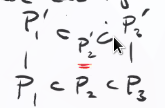
\includegraphics{figures/image_2020-09-10-10-18-40.png}
\caption{Image}
\end{figure}

In this process, the length of the chain decreased since \(\gens{0}\)
was deleted, but otherwise the chains are in bijective correspondence.
So the inductive hypothesis applies. \(\qed\)

\hypertarget{using-dimension-theory}{%
\subsection{Using Dimension Theory}\label{using-dimension-theory}}

Key fact used: the dimension doesn't change under integral extensions,
i.e.~if \(R\injects R'\) is integral then \(\dim R = \dim R'\).

\begin{claim}

Any affine variety has finite dimension.

\end{claim}

\begin{proof}

We have \(\dim X = \dim A(X)\), where \(A(X) \da \kx{n} I\) for some
\(I(X)=\sqrt{I(X)}\).

The noether normalization lemma (used in proof of nullstellensatz) shows
that a finitely generated \(k\dash\)algebra is an integral extension of
some polynomial ring \(k[y_1, \cdots, y_d]\). I.e., the following
extension is integral:
\begin{align*}  
k[y_1, \cdots, y_d] \injects k[x_1, \cdots, x_n]/I
.\end{align*}

We can conclude that \(\dim A(X) = d < \infty\).

\end{proof}

\begin{proposition}[?]

Let \(X, Y\) be irreducible affine varieties. Then

\begin{enumerate}
\def\labelenumi{\alph{enumi}.}
\tightlist
\item
  \(\dim X\cross Y = \dim X + \dim Y\).
\item
  \(Y\subset X \implies \dim X = \dim Y + \codim_X Y\).
\item
  If \(f\in A(X)\) is nonzero, then any component of \(V(f)\) has
  codimension 1.
\end{enumerate}

\end{proposition}

\begin{proof}

\begin{remark}

Why is \(X\cross Y\) again an affine variety? If \(X\subset \AA^n/k\),
\(Y\subset \AA^m/k\) with \(X = V(I), Y = V(J)\), then
\(X\cross Y \subset \AA^n/k \cross \AA^m/k = \AA^{n+m}/k\) can be given
by taking \(I+J \normal k[x_1, \cdots, x_n, y_1, \cdots, y_m]\) using
the natural inclusions of \(\kx{\ell}\).

Note that we can write
\begin{align*}  
k[x_1, \cdots, x_n, y_1, \cdots, y_m] = \kx{n} \tensor_k k[y_1, \cdots, y_n]
\end{align*} where we think of
\(x_i = x_i \tensor 1, y_j = 1 \tensor y_j\). We thus map \(I, J\) to
\(I\tensor 1 + 1\tensor J\) and obtain
\(V(I\tensor 1 + 1\tensor J) = X\cross Y\) and
\(A(X\cross Y) = A(X)\tensor_k A(Y)\).

In general, for \(k\dash\)algebras \(R,S\),
\begin{align*}  
R/I \tensor_k S/J \cong R\tensor_k S / \gens{I\tensor 1 + 1\tensor J}
.\end{align*}

\end{remark}

\begin{remark}

For \(R,S\) finitely generated \(k\dash\)algebras,
\(\dim R\tensor_k S = \dim R + \dim S\).

\end{remark}

Part (a) is proved by the above remarks.

For part (b), the statement is equivalent to \(P\subset A(X)\) with
\(I(Y) \subset P\) is a member of some maximal chain, along with the
statement that all maximal chains are the same length.

\end{proof}

\hypertarget{tuesday-september-15}{%
\section{Tuesday, September 15}\label{tuesday-september-15}}

\hypertarget{review}{%
\subsection{Review}\label{review}}

Let \(k=\bar k\), we're setting up correspondences
\begin{align*}  
\text{Ring Theory} 
\quad&\quad 
\text{Geometry/Topology of Affine Varieties}
\\
\text{Polynomial functions} 
\quad&\quad 
\text{Affine space} 
\\
k[x_1, \cdots, x_n]
\quad&\quad 
\AA^n/k \da \ts{\thevector{a_1, \cdots, a_n} \in k^n } 
\\
\text{Maximal ideals } \gens{x_1 - a_1, \cdots, x_n - a_n} 
\quad&\quad 
\text{Points } \thevector{a_1, \cdots, a_n} \in \AA^n/k
\\
\text{Radical ideals } I\normal k[x_1, \cdots, x_n]
\quad&\quad 
\text{Affine varieties } X\subset  \AA^n/k, \text{ vanishing locii of polynomials} 
\\
I &\mapsto V(I) \da \ts{a\st f(a) = 0 \forall f\in I} \\
I(X) \da \ts{f \st \restrictionof{f}{X} = 0} &\mapsfrom X 
\\
\text{Radical ideals containing $I(X)$, i.e. ideals in $A(X)$} 
\quad&\quad 
\text{closed subsets of $X$, i.e. affine subvarieties}
\\
A(X) \text{ is a domain}
\quad&\quad 
\text{$X$ irreducible}
\\
\text{$A(X)$ is not a direct sum}
\quad&\quad 
\text{$X$ connected} 
\\
\text{Prime ideals in }A(X)
\quad&\quad 
\text{Irreducible closed subsets of }X
\\
\text{Krull dimension $n$ (longest chain of prime ideals)}
\quad&\quad 
\dim X = n,\, \text{(longest chain of irreducible closed subsets)}
.\end{align*}

\begin{quote}
Recall that we defined the coordinate ring \(A(X) \da \kx{n} / I(X)\),
which contained no nilpotents.
\end{quote}

We had some results about dimension

\begin{enumerate}
\def\labelenumi{\arabic{enumi}.}
\tightlist
\item
  \(\dim X<\infty\) and \(\dim \AA^n = n\).
\item
  \(\dim Y + \codim_X Y = \dim X\) when \(Y\subset X\) is irreducible.
\item
  Only over \(\bar k = k\), \(\codim_X V(f) = 1\).
\end{enumerate}

\begin{example}

Take \(V(x^2+y^2) \subset \AA^2/\RR\)

\end{example}

\begin{definition}[?]

An affine variety \(Y\) of

\begin{itemize}
\tightlist
\item
  \(\dim Y = 1\) is a \textbf{curve},
\item
  \(\dim Y = 2\) is a \textbf{surface},
\item
  \(\codim_X Y = 1\) is a \textbf{hypersurface in \(X\)}
\end{itemize}

\end{definition}

Question: Is every hypersurface the vanishing locus of a \emph{single}
polynomials \(f\in A(X)\)?

Answer: This is true iff \(A(X)\) is a UFD.

\begin{definition}[Codimension in a Ring]

\(\codim_R \mfp\) is the length of the longest chain
\begin{align*}P_0 \subsetneq P_1 \subsetneq \cdots \subsetneq P_n = \mfp.\end{align*}

\end{definition}

Recall that \(f\) is irreducible if
\(f = f_1 f_2 \implies f_i \in R\units\) for one \(i\), and \(f\) is
prime iff \(\gens{f}\) is a prime ideal, or equivalently
\(f\divides ab \implies f\divides a\) or \(f\divides b\).

Note that prime implies irreducible, since \(f\) divides itself.

\begin{proposition}[?]

Let \(R\) be a Noetherian domain, then TFAE

\begin{enumerate}
\def\labelenumi{\alph{enumi}.}
\item
  All prime ideals of codimension 1 are principal.
\item
  \(R\) is a UFD.
\end{enumerate}

\end{proposition}

\begin{proof}

\(a\implies b\):

Let \(f\) be a nonzero non-unit, we'll show it admits a prime
factorization. If \(f\) is not irreducible, then \(f = f_1 f_1'\), both
non-units. If \(f_1'\) is not irreducible, we can repeat this, to get a
chain
\begin{align*}  
\gens{f} \subsetneq \gens{f_1'} \subsetneq \gens{f_2'} \subsetneq \cdots
,\end{align*} which must terminate.

This yields a factorization \(f = \prod f_i\) with \(f_i\) irreducible.
To show that \(R\) is a UFD, it thus suffices to show that the \(f_i\)
are prime. Choose a minimal prime ideal containing \(f\). We'll use
Krull's Principal Ideal Theorem: if you have a minimal prime ideal
\(\mfp\) containing \(f\), its codimension \(\codim_R \mfp\) is one. By
assumption, this implies that \(\mfp = \gens{g}\) is principal. But
\(g\divides f\) with \(f\) irreducible, so \(f,g\) differ by a unit,
forcing \(\mfp = \gens{f}\). So \(\gens{f}\) is a prime ideal.\\

\(b\implies a\):

Let \(\mfp\) be a prime ideal of codimension 1. If \(\mfp = \gens{0}\),
it is principal, so assume not. Then there exists some nonzero non-unit
\(f\in \mfp\), which by assumption has a prime factorization since \(R\)
is assumed a UFD. So \(f=\prod f_i\).

Since \(\mfp\) is a prime ideal and \(f\in\mfp\), some \(f_i\in \mfp\).
Then \(\gens{f_i} \subset \mfp\) and \(\mfp\) minimal implies
\(\gens{f_i} = \mfp\), so \(\mfp\) is principal.

\end{proof}

\begin{corollary}[?]

Every hypersurface \(Y\subset X\) is cut out by a single polynomial, so
\(Y=V(f)\), iff \(A(X)\) is a UFD.

\end{corollary}

\begin{example}

Apply this to \(R=A(X)\), we find that there is a bijection
\begin{align*}  
\codim 1 \text{ prime ideals}
\iff 
\codim 1 \text{ closed irreducible subsets }Y\subset X,\text{ i.e. hypersurfaces}
.\end{align*}

Taking \(A(X) = \CC[x,y,z]/\gens{x^2+y^2-z^2}\), whose real points form
a cone:

\begin{figure}
\centering
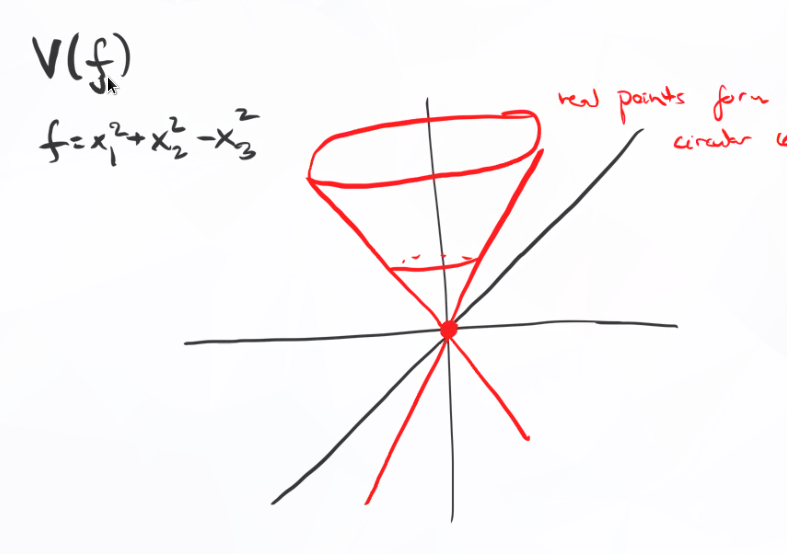
\includegraphics{figures/image_2020-09-15-10-26-24.png}
\caption{Image}
\end{figure}

Note that \(x^2 + y^2 = (x-iy)(x+iy) = z^2\) in this quotient, so this
is not a UFD.

Then taking a line through its surface is a codimension 1 subvariety not
cut out by a single polynomial. Such a line might be given by
\(V(x + iy, z)\), which is 2 polynomials, so why not codimension 2?

Note that \(V(z)\) is the union of the lines

\begin{itemize}
\tightlist
\item
  \(z = 0, x + iy= 0\),
\item
  \(z=0, x - iy = 0\).
\end{itemize}

Note that it suffices to show that this ring has an irreducible that is
not prime. Supposing \(z = f_1 f_2\), some \(f_i\) is a unit, then \(z\)
is not prime because \(z\divides xy\) but divides neither of \(x,y\).

\end{example}

\begin{example}

Note that \(\kx{n}\) is a UFD since \(k\) is a UFD. Applying the
corollary, every hypersurface in \(\AA^n\) is cut out by a single
irreducible polynomial.

\end{example}

\begin{definition}[?]

An affine variety \(X\) is of \textbf{pure dimension \(d\)} iff every
irreducible component \(X_i\) is of dimension \(d\).

\end{definition}

\begin{quote}
Note that \(X\) is a Noetherian space, so has a unique decomposition
\(X = \union X_i\).
\end{quote}

Given \(X\subset \AA^n/k\) of pure dimension \(n-1\), \(X = \union X_i\)
with \(X_i\) hypersurfaces with \(I(X_j) = \gens{f_j}\),
\(I(X) = \gens{f}\) where \(f = \prod f_i\).

\begin{definition}[?]

Given such an \(X\), define the \textbf{degree of a hypersurface} as the
degree of \(f\) where \(I(X) = \gens{f}\).

\end{definition}

\hypertarget{thursday-september-17}{%
\section{Thursday, September 17}\label{thursday-september-17}}

\hypertarget{regular-functions}{%
\subsection{Regular Functions}\label{regular-functions}}

\begin{quote}
See chapter 3 in the notes.
\end{quote}

Some examples:

\begin{itemize}
\tightlist
\item
  \(X\) a manifold or an open set in \(\RR^n\) has a ring of
  \(C^\infty\) functions.
\item
  \(X \subset \CC\) has a ring of holomorphic functions.
\item
  \(X\subset \RR\) has a ring of real analytic functions
\end{itemize}

These all share a common feature: it suffices to check if a function is
a member on an arbitrary open set about a point, i.e.~they are
\emph{local}.

\begin{definition}[?]

Let \(X\) be an affine variety and \(U\subseteq X\) open. A
\textbf{regular function} on \(U\) is a function \(\phi: U\to k\) such
that \(\phi\) is ``locally a fraction'', i.e.~a ratio of polynomial
functions.

More formally, for all \(p\in U\) there exists a \(U_p\) with
\(p\in U_p \subseteq U\) such that \(\phi(x) = g(x)/ f(x)\) for all
\(x\in U_p\) with \(f, g\in A(X)\).

\end{definition}

\begin{example}

For \(X\) an affine variety and \(f\in A(X)\), consider the open set
\(U\da V(f)^c\). Then \({1\over f}\) is a regular function on \(U\), so
for \(p\in U\) we can take \(U_p\) to be all of \(U\).

\end{example}

\begin{example}

For \(X = \AA^1\), take \(f=x-1\). Then \({x\over x-1}\) is a regular
function on \(\AA^1 \sm\ts{1}\).

\end{example}

\begin{example}

Let \(X + V(x_1 x_4 - x_2 x_3)\) and
\begin{align*}  
U \da X\sm V(x_2, x_4) = \ts{\thevector{x_1, x_2, x_3, x_4} \st x_1 x_4 = x_2 x_3, x_2\neq 0 \text{ or } x_4\neq 0 }
.\end{align*}

Define
\begin{align*}  
\phi: U &\to K \\
\thevector{x_1, x_2, x_3, x_4} &\mapsto
\begin{cases}
{x_1\over x_2} & \text{if } x_2 \neq 0 \\
{x_3\over x_4} & \text{if } x_4 \neq 0
\end{cases}
.\end{align*}

This is well-defined on \(\ts{x_2\neq 0} \intersect \ts{x_4 \neq 0}\),
since \({x_1\over x_2} = {x_3 \over x_4}\). Note that this doesn't
define an element of \(k\) at \(\thevector{0,0,0,1}\in U\). So this is
not globally a fraction.

\end{example}

Notation: we'll let \(\OO_X(U)\) is the ring of regular function on
\(U\).

\begin{proposition}[?]

Let \(U\subset X\) be an affine variety and \(\phi \in \OO_X(U)\). Then
\(V(\phi) \da \ts{x\in U \st \phi(x) = 0}\) is closed in the subspace
topology on \(U\).

\end{proposition}

\begin{proof}

For all \(a\in U\) there exists \(U_a\subset U\) such that
\(\phi = g_a/f_a\) on \(U_a\) with \(f_a, g_a \in A(X)\) with
\(f_a \neq 0\) on \(U_a\).

Then
\begin{align*}  
\ts{x\in U_a \st \phi(x) \neq 0} = U_a \sm V(g_a)\intersect U_a
\end{align*} is an open subset of \(U_a\), so taking the union over
\(a\) again yields an open set. But this is precisely \(V(\phi)^c\).

\end{proof}

\begin{proposition}

Let \(U\subset V\) be open in \(X\) an \emph{irreducible} affine
variety. If \(\phi_1, \phi_2 \in \OO_X(V)\) agree on \(U\), then they
are equal.

\end{proposition}

\begin{proof}

\(V(\phi_1 - \phi_2)\) contains \(U\) and is closed in \(V\). It
contains \(\bar U\intersect V\), by an earlier lemma, \(X\) irreducible
implies that \(\bar U = X\) and so \(V(\phi_1 - \phi_2) =V\).

\end{proof}

Compare and contrast: Let \(U\subset V \subset \RR^n\) be open. If
\(\phi_1, \phi_2 \in C^\infty(V)\) such that \(\phi_1, \phi_2\) are
equal when restricted \(U\subset V\). Does this imply
\(\phi_1 = \phi_2\)?

For \(\RR^n\), no, there exist smooth bump functions. You can make a
bump function on \(V\setminus U\) and extend by zero to \(U\). For
\(\CC\) and holomorphic functions, the answer is yes, by the uniqueness
of analytic continuation.

\begin{definition}[(Important) Distinguished Opens]

A \textbf{distinguished open set} in an affine variety is one of the
form
\begin{align*}  
D(f) \da X\sm V(f) = \ts{x\in X \st f(x) = 0}
.\end{align*}

\end{definition}

\begin{proposition}

The distinguished open sets form a base of the zariski topology.

\end{proposition}

\begin{proof}

Given \(f, g\in A(X)\), we can check:

\begin{enumerate}
\def\labelenumi{\arabic{enumi}.}
\tightlist
\item
  Closed under finite intersections: \(D(f) \intersect D(g) = D(fg)\).
\item

  \begin{align*}U = X\sm V(f_1, \cdots, f_k) = V\sm \bigcap V(f_i) = \bigcup D(f_i),\end{align*}
  and any open set is a \emph{finite} union of distinguished opens by
  the Hilbert basis theorem.
\end{enumerate}

\end{proof}

\begin{proposition}[?]

The regular functions on \(D(f)\) are given by
\begin{align*}  
\OO_X(D(f)) = \ts{{ g \over f^n} \st g\in A(X), n\in \NN} = A(X)_{\gens{f}}
,\end{align*} the localization of \(A(X)\) at \(\gens{f}\).

\end{proposition}

Note that if \(f=1\), then \(\OO_X(X) = A(X)\).

\begin{proposition}[?]

Note that \({g\over f^n} \in \OO_X(D(f))\) since \(f^n\neq 0\) on
\(D(f)\). Let \(\phi: D(f) \to k\) be a regular function. By definition,
for all \(a\in D(f)\) there exists a local representation as a fraction
\(\phi = g_a/f_a\) on \(U_a\ni a\). Note that \(U_a\) can be covered by
distinguished opens, one of which contains \(a\). Shrink \(U_a\) if
necessary to assume it is a distinguished open set \(U_a = D(h_a)\).\\

Now replace
\begin{align*}  
\phi = {g_a \over f_a} = {g_a h_a \over f_a h_a}
,\end{align*} which makes sense because \(h_a\neq 0\) on \(U_a\). We can
assume wlog that \(h_a = f_a\). Why? We have \(\phi = {g_a \over f_a}\)
on \(D(f_a)\). Since \(f_a\) doesn't vanish on \(U_a\), we have
\(V(f_a h_a) = V(h_a)\) since \(V(f_a) \subset D(h_a)^c = V(h_a)\).

Consider \(U_a = D(f_a)\) and \(U_b = D(f_b)\), on which
\(\phi = {g_a\over f_a}\) and \(\phi = {g_b \over f_b}\) respectively.
On \(U_a\intersect U_b = D(f_a f_b)\), these are equal,
i.e.~\(f_b g_a = f_a g_b\) in the coordinate ring \(A(X)\).\\

Then \(D(f) = \bigcup_a D(f_a)\), so take the component
\(V(f) = \intersect V(f_a)\) by the Nullstellensatz
\(f\in I(V(f_a)) = I(V(g_a, a\in D_f)) = \sqrt{f_a \st a\in D_f}\).

Then there exists an expression \(f^n = \sum k_a f_a\) as a finite sum,
so set \(g - \sum g_a k_a\).

\begin{claim}

\(\phi = g/f^n\) on \(D(f)\).\\

This follows because on \(D(f_b)\), we have \(\phi = {g_b \over f_b}\),
and so \(gf_b = \sum k_a g_a f_b\).

\end{claim}

\begin{quote}
Finish next class
\end{quote}

\end{proposition}

\hypertarget{tuesday-september-22}{%
\section{Tuesday, September 22}\label{tuesday-september-22}}

\hypertarget{review-regular-functions}{%
\subsection{Review: Regular Functions}\label{review-regular-functions}}

Given an affine variety \(X\) and \(U\subseteq X\) open, a \emph{regular
function} \(\phi: U\to k\) is one locally (wrt the zariski topology) a
fraction. We write the set of regular functions as \(\OO_X\).

\begin{example}

\(X = V(x_1 x_4 - x_2 x_3)\) on \(U = V(x_2, x_4)^c\), the following
function is regular:
\begin{align*}  
\phi: U &\to k \\
x &\mapsto 
\begin{cases}
{x_1\over x_2} & x_2 \neq 0 \\ \\
{x_3 \over x_4} & x_4 \neq 0
\end{cases}
.\end{align*} Note that this is not globally a fraction.

\end{example}

\begin{definition}[Distinguished Open Sets]

A \emph{distinguished open set} \(D(f) \subseteq X\) for some
\(f\in A(X)\) is \(V(f)^c \da \ts{x\in X \st f(x) \neq 0}\).

\end{definition}

These are useful because the \(D(f)\) form a base for the zariski
topology.

\begin{proposition}[?]

For \(X\) an affine variety, \(f\in A(X)\), we have
\begin{align*} 
\OO_X(D(f)) = \ts{ {g\over f^n} \st g\in A(X), n\in \NN}
.\end{align*}

\end{proposition}

\begin{proof}

The first reduction we made was that \(\phi \in \OO_X(D(f))\) is
expressible as \(g_a\over f_a\) on distinguished opens \(D(f_a)\)
covering \(D(f)\). We also noted that
\begin{align*}
{g_a \over f_a} = {g_b \over f_b} \text{ on } D(f_a) \intersect D(f_b) \implies f_b g_a = f_a g_b \text{ in } A(X)
.\end{align*}\\

The second step was writing \(D(f) = \union D(f_a)\), and so
\(V(f) = \intersect_a V(f_a)\) implies that
\(f\in I(V(\ts{f_a \st a\in U}))\). By the Nullstellensatz,
\(f\in \sqrt{\gens{f_a \st a\in U}}\), so \(f^N = \sum k_a f_a\) for
some \(N\). So construct \(g = \sum k_a g_a\), then compute
\begin{align*}  
gf_b = \sum_a k_a g_a f_b = \sum_a k_a g_b f_a = g_b \sum k_a f_a = g_b f^N
.\end{align*} Thus \(g/f^N = g_b / f_b\) for all \(b\), and we can thus
conclude
\begin{align*}  
\phi \da \ts{{g_b \over f_b} \text{ on } D(f_b)} = g/f^N
.\end{align*}

\end{proof}

\begin{corollary}[?]

For \(X\) an affine variety, \(\OO_X(X) = A(X)\).

\end{corollary}

\begin{warning}

For \(k\) not algebraically closed, the proposition and corollary are
both false. Take \(X = \AA^1/\RR\), then \({1\over x^2+1} \in \RR(x)\),
but \(\OO_X(X) \neq A(X) = \RR[x]\).

\end{warning}

\begin{definition}[Localization]

Let \(R\) be a ring and \(S\) a set closed under multiplication, then
the localization at \(S\) is defined by
\begin{align*}  
R_S \da \ts{r/s \st r\in R, s\in S} / \sim
.\end{align*} where
\(r_1/s_1 \sim r_2/s_2 \iff s_3(s_2 r_1 - s_1 r_2) = 0\) for some
\(s_3 \in S\).

\end{definition}

\begin{example}

Let \(f\in R\) and take \(S = \ts{f^n \st n\geq 1}\), then
\(R_f \da R_S\).

\end{example}

\begin{corollary}[?]

\(\OO_X(D(f)) = A(X)_f\) is the localization of the coordinate ring.

\end{corollary}

These requires some proof, since the LHS literally consists of functions
on the topological space \(D(f)\) while the RHS consists of formal
symbols.

\begin{proof}

Consider the map
\begin{align*}  
A(X)_f &\to \OO_X(D(f)) \\
``g/f^n" &\mapsto g/f^n: D(f) \to k
.\end{align*}

By definition, there exists a \(k\geq 0\) such that
\begin{align*}  
f^k(f^m g - f^n g') = 0 
\implies
f^k(f^m g - f^n g') = 0 \text{ as a function on } D(f)
.\end{align*} Since \(f^k \neq 0\) on \(D(f)\), we have
\(f^m g = f^n g'\) as a function on \(D(f)\), so \(g/f^n = g'/g^m\) as
functions on \(D(f)\).\\

\textbf{Surjectivity}: By the proposition, we have surjectivity,
i.e.~any element of \(|OO_x(D(f))\) can be represented by some
\(g/f^n\).\\

\textbf{Injectivity}: Suppose \(g/f^n\) defines the zero function on
\(D(f)\), then \(g = 0\) on \(D(f)\) implies that \(fg=0\) on \(X\)
(i.e.~\(fg= 0 \in A(X)\)), and we can write
\(f(g\cdot 1 - f^n\cdot 0) = 0\). Then \(g/f^n\sim 0/1 \in A(X)_f\),
which forces \(g/f^n = 0\in A(X)_f\).

\end{proof}

\hypertarget{sheaves}{%
\subsection{Sheaves}\label{sheaves}}

Idea: spaces on functions on topological spaces.

\begin{definition}[Presheaf]

A \emph{presheaf} (of rings) \(\mathcal{F}\) on a topological space is

\begin{enumerate}
\def\labelenumi{\arabic{enumi}.}
\item
  For every open set \(U\subset X\) a ring \(\mathcal{F}(U)\).
\item
  For any inclusion \(U\subset V\) a restriction map
  \(\res_{VU}: \mathcal{F}(V) \to \mathcal{F}(U)\) satisfying
\end{enumerate}

\begin{enumerate}
\def\labelenumi{\alph{enumi}.}
\tightlist
\item
  \(F(\emptyset) = 0\).
\item
  \(\res_{UU} = \id_{\mathcal{F}(U)}\).
\item
  \(\res_{VW} \circ \res_{UV} = \res_{UW}\).
\end{enumerate}

\end{definition}

\begin{example}

The smooth functions on \(\RR\) with the standard topology,
\(\mathcal{F} = C^\infty\) where \(C^\infty(U)\) is the set of smooth
functions \(U\to \RR\). It suffices to check the restriction condition,
but the restriction of a smooth function is smooth: if \(f\) is smooth
on \(U\), it is smooth at every point in \(U\), i.e.~all derivatives
exist at all points of \(U\). So if \(V\subset U\), all derivatives of
\(f\) will exist at points \(x \in V\), so \(f\) will be smooth on
\(V\).

Note that this also works with continuous functions.

\end{example}

\begin{definition}[Sheaf]

A \emph{sheaf} is a presheaf satisfying an additional gluing property:
given \(\phi_i \in \mathcal{F}(U_i)\) such that
\(\restrictionof{\phi_i}{U_i\intersect U_j} = \restrictionof{\phi_j}{U_i \intersect U_j}\),
then there exists a unique \(\phi\in \mathcal{F}(\union_i U_i)\) such
that \(\restrictionof{\phi}{U_i} = \phi_i\).

\end{definition}

\hypertarget{thursday-september-24}{%
\section{Thursday, September 24}\label{thursday-september-24}}

Recall that we defined the \emph{regular functions} \(\OO_X(U)\) on an
open set \(U\subset X\) an affine variety as the set of functions
\(\phi: U\to k\) such that \(\phi\) is locally a fraction, i.e.~for all
\(p\in U\) there exists a neighborhood of \(p\), say \(U_p \subset U\),
such that \(\phi\) restricted to \(U_p\) is given by \(g_p \over f_p\)
for some \(f_p, g_p \in A(X)\).

We proved that on a distinguished open set \(D(f) = V(f)^c\), we have
\(\OO_X(D(f)) = A(X)_f\). An important example was that
\(\OO_X(X) = A(X)\).

Question: If \(X\) is a variety over \(\CC\), does \(A(X) = \Hol(X)\)?
The answer is no, since taking \(\AA^1/\CC \cong \CC = X\) we obtain
\(A(X) = \CC[x]\) but for example \(e^z \in \Hol(X)\).

On the other hand, if you require that \(f\in \Hol(X)\) is meromorphic
at \(\infty\), i.e.~\(f({1\over z})\) is meromorphic at zero, then you
do get \(\CC[z]\). This is an example of GAGA!

\begin{quote}
Review: what is a category?
\end{quote}

\begin{quote}
Review: what is a presheaf?
\end{quote}

\hypertarget{tuesday-september-29}{%
\section{Tuesday, September 29}\label{tuesday-september-29}}

Recall the definition of a presheaf: a sheaf of rings on a space is a
contravariant functor from its category of open sets to ring, such that

\begin{enumerate}
\def\labelenumi{\arabic{enumi}.}
\tightlist
\item
  \(F(\emptyset) = 0\)
\item
  The restriction from \(U\) to itself is the identity,
\item
  Restrictions compose.
\end{enumerate}

Examples:

\begin{itemize}
\tightlist
\item
  Smooth functions on \(\RR^n\)
\item
  Holomorphic functions on \(\CC\)
\end{itemize}

Recall the definition of sheaf: a presheaf satisfying \emph{unique}
gluing: given \(f_i \in \mathcal{F}(U_i)\), such that
\(\restrictionof{f_i}{U_i \intersect U_j} = \restrictionof{f_j}{U_i\intersect U_j}\)
implies that there exists a unique \(f\in \mathcal{F}(\union U_i)\) such
that \(\restrictionof{f}{U_i} = f_i\).

Question: Are the constant functions on \(\RR\) a presheaf and/or a
sheaf?

Answer: This is a presheaf but not a sheaf. Set
\(\mathcal{F}(U) = \ts{f: U\to \RR \st f(x) = c} \cong \RR\) with
\(\mathcal{F}(\emptyset) = 0\). Can check that restrictions of constant
functions are constant, the composition of restrictions is the overall
restriction, and restriction from \(U\) to itself gives the function
back.

Given constant functions \(f_i \in \mathcal{F}(U_i)\), does there exist
a unique constant function \(\mathcal{F}(\union U_i)\) restricting to
them? No: take \(f_1 = 1\) on \((0, 1)\) and \(f_2 = 2\) on \((2, 3)\).
Can check that they both restrict to the zero function on the
intersection, since these sets are disjoint.

How can we make this into a sheaf? One way: weaken the topology. Another
way: define another presheaf \(\mathcal{G}\) on \(\RR\) given by
\emph{locally} constant function,
i.e.~\(\ts{f: U\to \RR \st \forall p\in U, \exists U_p\ni p,\, \ro{f}{U_p} \text{ is constant}}\).
Reminiscent of definition of regular functions in terms of local
properties.

\begin{example}

Let \(X = \ts{p, q}\) be a two-point space with the discrete topology,
i.e.~every subset is open. Then define a sheaf by
\begin{align*}  
\emptyset &\mapsto 0 \\
\ts{p} &\mapsto R \\
\ts{q} &\mapsto S \\
\implies \ts{p, q} &\mapsto R\cross S
,\end{align*} where the sheaf condition forces the assignment of the
whole space to be the product. Note that the first 3 assignments are
automatically compatible, which means that we need a unique
\(f\in \mathcal{F}(X)\) restricting to \(R\) and \(S\). In other words,
\(\mathcal{F}(X)\) needs to be unique and have maps to \(R, S\), but
this is exactly the universal property of the product.

\end{example}

\begin{example}

Consider the presheaf on \(X\) given by
\(\mathcal{F}(X) = R\cross S \cross T\). Taking \(T = \ZZ/2\ZZ\), we can
force uniqueness to fail: by projecting to \(R, S\), there are two
elements in the fiber, namely \((r,s,0)\mapsto r,s\) and
\((r,s,1)\mapsto r,s\).

\end{example}

\begin{example}

Let \(X = \ts{a, b, c}\) and
\(\tau = \ts{\emptyset, \ts{a}, \ts{a, b}, \ts{a, c}}\). Can check that
it's closed under finite intersections and arbitrary unions, so this
forms a topology. Now make the assignments
\begin{align*}  
\ts{a}& \mapsto A \\
\ts{b}& \mapsto B \\
\ts{a, b}& \mapsto C \\
X &\mapsto ?
.\end{align*}

We have a situation like this:

\begin{center}\includesvg[width=\linewidth]{67688d82b4330cae60761458ca45d6ff13629a54}\end{center}

Unique gluing says that given \(r\in B, s\in C\) such that
\(\phi_B(r) = \phi_C(s)\), there should exist a unique
\(t\in \mathcal{F}(X)\) such that \(\ro{t}{\ts{a, b}} = r\) and
\(\ro{t}{\ts{a, c}} = s\). This recovers exactly the fiber product.
\begin{align*}  
B \cross_A C \da \ts{(r, s) \in B\cross C \st \phi_B(r) = \phi_C(s) \in A}
.\end{align*}

\end{example}

\begin{example}

Let \(X\) be an affine variety with the Zariski topology and let
\(\mathcal{F} \da \OO_X\) be the sheaf of regular functions:
\begin{align*}  
\OO_X(U) \da \ts{f: U\to k \st \forall p\in U,\, \exists U_p \ni p,\,\, \ro{f}{U_p} ={g_p \over h_p} }
.\end{align*}

Is this a presheaf? We can check that there are restriction maps:
\begin{align*}  
\OO_X(U) &\to \OO_X(V) \\
\ts{f: U\to K} &\mapsto \ts{\ro{f}{V}(x) \da f(x) \text{ for } x \in V }
.\end{align*} This makes sense because if \(V\subset U\), any \(x\in V\)
is in the domain of \(f\). Given that \(f\) is locally a fraction, say
\(\rho = g_p / h_p\) on \(U_p \ni p\), is \(\ro{\phi}{V}\) locally a
fraction? Yes: for all \(p\in V\subset U\), \(\phi = g_p / f_p\) on
\(U_p\) and this remains true on \(U_p \intersect V\).

To check that \(\OO_X\) is a sheaf, given a set of regular functions
\(\ts{\phi_i: U_i \to k}\) agreeing on intersections, define
\begin{align*}  
\phi: \union U_i &\to k\\
\phi(x) &\da \phi_i(x) \text{ if }x\in U_i
.\end{align*}

This is well-defined, since if \(x\in U_i \intersect U_j\),
\(\phi_i(x) = \phi_j(x)\) since both restrict to the same function on
\(U_i \intersect U_j\) by assumption.

Why is \(\phi\) locally a fraction? We need to check that for all
\(p\in U \da \union U_i\) there exists a \(U_p \ni p\) with
\(\ro{\phi}{U_p} = g_p/h_p\). But any \(p\in \union U_i\) implies
\(p\in U_i\) for some \(i\). Then there exists an open set
\(U_{i, p} \ni p\) in \(U_i\) such that
\(\ro{\phi}{U_{i, p}} = g_p / h_p\) by definition of a regular function.
So take \(U_p = U_{i, p}\) and use the fact that
\(\ro{\phi}{U_i} = \phi_i\) along with compatibility of restriction.

\end{example}

\begin{remark}

General observation: any presheaf of functions is a sheaf when the
functions are defined by a local property, i..e any property that can be
checked at \(p\) by considering an open set \(U_p \ni p\).

As in the examples of smooth or holomorphic functions, these were local
properties. E.g. checking that a function is smooth involves checking on
an open set around each point. On the other hand, being a constant
function is not a local property.

\end{remark}

\begin{definition}[Restriction of a (Pre)sheaf]

Given a sheaf \(\mathcal{F}\) on \(X\) and an open set \(U\subset X\),
we can define a sheaf \(\ro{\mathcal{F}}{U}\) on \(U\) (with the
subspace topology) by defining
\(\ro{\mathcal{F}}{U}(V) \da \mathcal{F}(V)\) for \(U\subseteq V\).

\end{definition}

\begin{definition}[Stalks]

Let \(\mathcal{F}\) be a sheaf on \(X\) and \(p\in X\) a point. The
\emph{stalk} of \(\mathcal{F}\) at \(p\), denoted \(\mathcal{F}_p\) for
\(p\in U\), is defined by
\begin{align*}  
\mathcal{F}_p \da \ts{(U, \phi) \st \phi \in \mathcal{F}(U) } / \sim
\end{align*} where \((U, \phi) \sim (V, \phi')\) iff there exists a
\(W\subset U\intersect V\) and \(p\in W\) such that
\(\ro{\phi}{W} = \ro{\phi}{W}'\).

\end{definition}

\begin{example}

What is the stalk of \(\Hol(\CC)\) at \(p=0\)?

Examples of equivalent elements in this stalk:

\begin{figure}
\centering
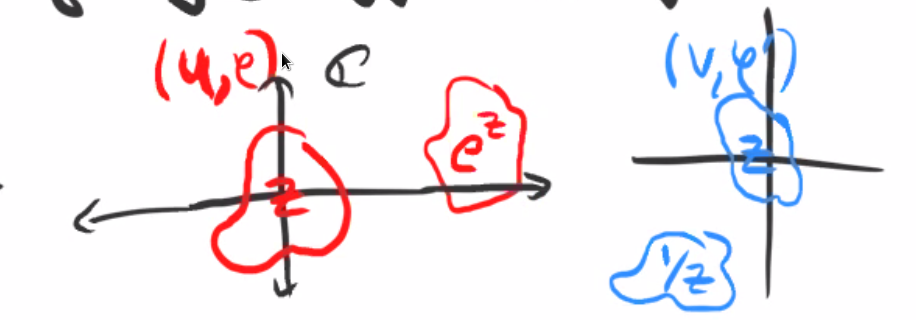
\includegraphics{figures/image_2020-09-29-10-38-22.png}
\caption{O}
\end{figure}

In this case
\begin{align*}  
\Hol(\CC)_0 = \ts{\phi = \sum_{i>0}c_i z^i \st \phi \text{ has a positive radius of convergence}}
.\end{align*}

\end{example}

\begin{definition}[Sections]

An element \(f\in \mathcal{F}(U)\) is called a \emph{section} over
\(U\), and elements of the stalk \(f\in \mathcal{F}_p\) are called
\emph{germs} at \(p\).

\end{definition}

\hypertarget{thursday-october-01}{%
\section{Thursday, October 01}\label{thursday-october-01}}

\hypertarget{stalks-and-localizations}{%
\subsection{Stalks and Localizations}\label{stalks-and-localizations}}

Recall that a sheaf of rings on a topological space \(X\) is a ring
\(\mathcal{F}(U)\) for all open sets \(U\subset X\) satisfying four
properties:

\begin{enumerate}
\def\labelenumi{\arabic{enumi}.}
\item
  The empty set is mapped to zeor.
\item
  The morphism \(\mathcal{F}(U)\to \mathcal{F}(U)\) is the identity.
\item
  Given \(W\subset V\subset U\) we have
\item
  Gluing: given sections \(s_i \in\mathcal{F}(U_i)\) which agree on
  overlaps (restrict to the same function on \(U_i\intersect U_j\)),
  there is a unique \(s\in \mathcal{F}(\union U_i)\).
\end{enumerate}

\begin{example}

If \(X\) is an affine variety with the zariski topology,
\(\mathcal{O}_X\) is a sheaf of regular functions, where we recall
\(\mathcal{O}_X(U)\) are the functions \(\phi: U\to k\) that are locally
a fraction.

\end{example}

Recall that the \emph{stalk} of a sheaf \(\mathcal{F}\) at a point
\(p\in X\), is defined as
\begin{align*}  
\mathcal{F}_p \da \ts{(U, \phi) \st p\in U \text{ open },\, \phi \in \mathcal{F}(U)}/\sim
.\end{align*} where \((U, \phi) \sim (U', \phi')\) if there exists a
\(p\in W \subset U\intersect U'\) such \(\phi, \phi'\) restricted to
\(W\) are equal.

Recall that a \emph{local ring} is a ring with a unique maximal ideal
\(\mfm\). Given a prime ideal \(\mfp \in R\), so
\(ab\in \mfp \implies a,b\in \mfp\), the complement \(R\setminus P\) is
closed under multiplication. So we can localize to obtain
\(R_\mfp = \ts{a/s \st s\in R\setminus P, a\in R}/\sim\) where
\(a'/s' \sim a/s\) iff there exists a \(t\in R\sm P\) such that
\(t(a's - as') = 0\).

\begin{warning}

Note that \(R_f\) is localizing at the powers of \(f\), whereas
\(R_\mfp\) is localizing at the \emph{complement} of \(\mfp\).

\end{warning}

Since maximal ideals are prime, we can localize any ring \(R\) at a
maximal ideal \(R_\mfm\), and this will be a local ring. Why? The ideals
in \(R_\mfm\) biject with ideals in \(R\) contained in \(\mfm\). Thus
all ideals in \(R_\mfm\) are contained in the maximal ideal generated by
\(\mfm\), i.e.~\(\mfm R_\mfm\).

\begin{lemma}[?]

Let \(X\) be an affine variety. The stalk of the sheaf of regular
functions \(\OO_{X, p} \da (\OO_X)_p\) is isomorphic to the localization
\(A(X)_{\mfm_p}\) where \(\mfm_p \da I(\ts{p})\).

\end{lemma}

\begin{proof}

We can write
\begin{align*}  
A(X)_{\mfm_p} \da \ts{{g\over f} \st g\in A(X),\, f\in A(X)\sm \mfm_p} / \sim \\
\text{ where } g_1/f_1 \sim g_2/f_2 \iff \exists h(p) \neq 0 \text{ where }0 = h(f_2 g_1 - f_1 g_2)
.\end{align*} where the \(f\) are regular functions on \(X\) such that
\(f(p) = 0\).

We can also write
\begin{align*}  
\OO_{X, p} \da \ts{(U, \phi) \st p\in U,\, \phi \in \OO_X(U) } /\sim 
\\ \text{ where } (U, \phi) \sim (U', \phi') 
\iff \exists p\in W \subset U\intersect U' \text{ s.t. } \ro{\phi}{W} = \ro{\phi'}{W}
.\end{align*}

So we can define a map
\begin{align*}  
\Phi: A(X)_{\mfm_p} &\to \OO_{X, p} \\
{g\over f} &\mapsto \qty{D_f, {g\over f}}
.\end{align*}

\textbf{Step 1:} There are equivalence relations on both sides, so we
need to check that things are well-defined.

We have
\begin{align*}  
g/f \sim g'/f' &\iff \exists g \text{ such that } h(p) \neq 0,\, h(gf' - g'f)=0 \in A(X) \\
&\iff \text{the functions } {g\over f}, {g' \over f'} \text{ agree on } W\da D(f) \intersect D(f') \intersect D(h) \\
&\implies (D_f, g/f) \sim (D_{f'}, g'/f')
,\end{align*} since there exists a \(W\subset D_f \intersect D_{f'}\)
such that \(g/f, g'/f'\) are equal.\\

\textbf{Step 2:} Surjectivity, since this is clearly a ring map with
pointwise operations.

Any germ can be represented by \((U, \phi)\) with \(\phi \in \OO_X(U)\).
Since the sets \(D_f\) form a base for the topology, there exists a
\(D_f\subset U\) containing \(p\). By definition,
\((U, \phi) = (D_f, \ro{\phi}{D_f})\) in \(\OO_{X, p}\).

Using the proposition that \(\OO_X(D(f)) = A(X)_f\), this implies that
\(\ro{\phi}{D_f} = g/f^n\) for some \(n\) and \(f(p) \neq 0\), so
\((U, \phi)\) is in the image of \(\Phi\).\\

\textbf{Step 3}: Injectivity. We want to show that \(g/f\mapsto 0\)
implies that \(g/f = 0 \in A(X)_{\mfm_p}\).

Suppose that \((D_f, g/f) = 0 \in \OO_{X, p}\) and
\((U, \phi) = 0 \in \OO_{X,p}\), then there exists an open
\(W\subset D_f\) containing \(p\) such that after passing to some
distinguished open \(D_h\ni p\) such that \(\phi = 0\) on \(D_h\). Wlog
we can assume \(\phi = 0\) on \(U\), since we could shrink \(U\)
(staying in the same equivalence class) to make this true otherwise.
Then \(\phi = g/f\) on \(D_h\), using that \(\OO_X(D_f) = A(X)_f\), so
\(g/f = 0\) here. So there exists a \(k\) such that
\(f^k(g\cdot 1 - 0\cdot f) = 0\) in \(A(X)\), so
\(f^k g=0 \in A(X)_{\mfm_p}\).

\end{proof}

Conclusion:
\begin{align*}  
\OO_{X, p} \cong A(X)_{\mfm_p}
.\end{align*}

\begin{example}

Let \(X = \ts{p, q}\) with the discrete topology with the sheaf
\(\mathcal{F}\) given by \(p\mapsto R, q\mapsto S, X\mapsto R\cross S\).

Then \(\mathcal{F}_p = R\), since if \(U\) is open and \(p\in\ U\) then
either \(U= \ts{p}\) or \(U = X\). We can check that for \((r, s)\) a
section of \(\mathcal{F}\), we have an equivalence of germs
\((X, (r, s)) \sim (\ts{p}, r)\) since
\(\ts p \subset X\intersect \ts p\). Here \(X\) plays the role of \(U\),
\(\ts p\) of \(U'\), and the last \(\ts p\) the role of
\(W \subset U\intersect U'\).

\begin{align*}  
\OO_{X, p} &\to A(X) \\
(\ts{p}, r) &\mapsto r \\
\mathcal{F}_p &\cong R
.\end{align*}

\end{example}

\begin{example}

Let \(M\) be a manifold and consider the sheaf \(C^\infty\) of smooth
functions on \(M\). Then the stalk \(C_p^\infty\) at \(p\) is defined as
the set of smooth functions in a neighborhood of \(p\) modulo functions
being equivalent if they agree on a small enough ball \(B_\eps(p)\).
This contains a maximal ideal \(\mfm_p\), the smooth functions vanishing
at \(p\).

Then \(\mfm_p^2\) is again an ideal, equal to the set
\(\ts{f \st \del_i \del_j f\mid_p = 0,\, \forall i,j}\). Thus
\(\mfm_p/\mfm_p^2 \cong \ts{\del_v}\dual\), the dual of the set of
directional derivatives.

\end{example}

\hypertarget{whats-the-point}{%
\subsection{What's the Point!}\label{whats-the-point}}

Problem: what should a map of affine varieties be? A bad definition
would be just taking the continuous maps: for example, any bijection
\(\AA_\CC^1\) is a homeomorphism in the zariski topology. Why? This
coincides with the cofinite topology, and the preimage of a cofinite set
is cofinite.

How do we fix this?

\begin{enumerate}
\def\labelenumi{\arabic{enumi}.}
\item
  \(f:X\to Y\) is continuous, i.e.~\(f^{-1} (U)\) is open whenever \(U\)
  is open.
\item
  Given \(U\subset Y\) open and \(\phi \in \OO_Y(U)\), the function
  \(\phi \circ f: f^{-1}(U) \to k\) is regular.
\end{enumerate}

We'll take this to be the definition of a morphism \(X\to Y\).

\begin{example}

For smooth manifolds, we also require that there is a pullback that
preserves smooth functions:
\begin{align*}  
f^*: C^\infty(U) \to C^\infty(f^{-1}(U))
.\end{align*}

\end{example}

\hypertarget{tuesday-october-06}{%
\section{Tuesday, October 06}\label{tuesday-october-06}}

Note: the sheaf of locally constant functions valued in a set \(S\) is
written \(\underline{\mathbf S}\).

\hypertarget{gathmann-chapter-4}{%
\subsection{Gathmann Chapter 4}\label{gathmann-chapter-4}}

\begin{definition}[Ringed Spaces]

A \textbf{ringed space} is a topological space \(X\) together with a
sheaf \(\OO_X\) of rings.

\end{definition}

\begin{example}

\hfill

\begin{enumerate}
\def\labelenumi{\arabic{enumi}.}
\item
  \(X\) an affine variety and \(\OO_X\) its ring of regular functions.
\item
  \(X\) a manifold over \(\RR^n\) with \(\OO_X\) a ring of smooth or
  continuous functions on \(X\).
\item
  \(X = \ts{p, q}\) with the discrete topology and \(\OO_X\) given by
  \(p\mapsto R, q\mapsto S\).
\item
  Let \(U\subset X\) an open subset of \(X\) an affine variety. Then
  declare \(\OO_U\) to be \(\ro{OO_X}{U}\).
\end{enumerate}

\end{example}

Recall that the restriction of a sheaf \(\mathcal{F}\) to an open subset
\(U\subset X\) is defined by
\(\ro{\mathcal{F}}{U}(V) = \mathcal{F}(V)\).

\begin{example}

Let \(X\) be a topological space and \(p\in X\) a point. The
\emph{skyscraper sheaf at \(p\)} is defined by
\begin{align*}  
K_p(U) \da 
\begin{cases}
K & p\in U \\
0 & p\not\in U
\end{cases}
.\end{align*}

\end{example}

Convention: we'll always assume that \(\OO_X\) is a sheaf of functions,
so \(\OO_X(U)\) is a subring of all \(K\dash\)valued functions on \(U\).
Moreover, \(\res_{UV}\) is restriction of \(K\dash\)valued functions.

\begin{definition}[Morphisms]

A \emph{morphism of ringed spaces}
\begin{align*}  
(X, \OO_X) \mapsvia{f}  (Y, \OO_Y)
\end{align*} is a continuous map \(X\to Y\) such that for all opens
\(U \subset Y\) and any \(\phi \in \OO_Y(U)\), the pullback satisfies
\(f^* \phi \in \OO_X(f\inv(U))\), i.e.~the pullback of a regular
function is regular.

\end{definition}

Note: need convention that \(\OO_X\) is a sheaf of \(K\dash\)valued
functions in order to make sense of pullbacks. In general, for schemes,
need some analog of \(f^*: \OO_X(V) \to \OO_X(U)\).

\begin{example}

If \((X, \OO_X)\) is a ringed space associated to an affine variety, ?

\end{example}

\begin{example}

Let \(X = \AA^1/K\) and \(U = D(f)\) for \(f(x) =x\), then
\(D(f) = \AA^1\smz\). Then \(U\injects X\) is continuous. Given an open
set \(D(f) \subset \AA^1\), we have
\begin{align*}  
\OO_{\AA^1}(D(f)) \da \ts{g/f^n \st g\in K[x]}
.\end{align*} We want to show that
\(\iota: (U, \OO_U) \injects (X, \OO_X)\) is a morphism of ringed spaces
where \(\OO_U(V) = \OO_X(V)\). Does \(\iota^*\) pull back regular
functions to regular functions? Yes, since \(\iota^{-1} (D(f)) = D(xf)\)
and \(g/f^n \in \OO_U(\iota^{-1}(D(f)))\).

\end{example}

\begin{example}

A non-example: take
\begin{align*}  
h: \AA^1 &\to \AA^1 \\
x & \mapsto 
\begin{cases}
x & x \neq \pm 1 \\
-x & x= \pm 1
\end{cases}
.\end{align*} This is continuous because the zariski topology on
\(\AA^1\) is the cofinite topology (since the closed sets are finite),
so any injective map is continuous since inverse images of cofinite sets
are again cofinite.

Question: Does \(h\) define a morphism of ringed spaces? I.e., is the
pullback of a regular function on an open still regular? Take
\(U = \AA^1\) and the regular function \(x\in \OO_{\AA^1}(\AA^1)\). Then
\(h^*x = x\circ h\), so
\begin{align*}  
(x\circ h)(p) =
\begin{cases}
p & p\neq \pm 1 \\
-p & p= \pm 1 
\end{cases}
\not \in K[x]
\end{align*} since this is clearly not a polynomial: if two polynomials
agree on an infinite set of points, they are equal.

\end{example}

\begin{example}

Consider \(\iota: (\RR^2, C^\infty) \injects (\RR^3, C^\infty)\) is the
inclusion of a coordinate hyperplane. To say that this is a morphism of
ringed spaces, we need that for all \(U\subset \RR^3\) open and
\(f:U\to \RR\) a smooth function, we want
\(i^* f\in C^\infty (\iota^{-1}(U))\). But this is the same as
\(f\circ \iota \in C^\infty(\RR^2\intersect U)\), which is true.

\end{example}

\begin{proposition}[Properties of Morphisms of Ringed Spaces]

\hfill

\begin{enumerate}
\def\labelenumi{\arabic{enumi}.}
\item
  They can be composed: if \(\phi \in \OO_Z(U)\), then
  \(g^* \phi \in \OO_Y(g^{-1}(U))\) and so
  \(f^* g^* \phi \in \OO_X(f^{-1} g^{-1} (U))\).
\item
  The identity is a morphism.
\end{enumerate}

Thus ringed spaces form a category, since composition is associative.

\end{proposition}

\begin{lemma}[Gluing for Morphisms]

Let \(f:X\to Y\) be a continuous map between ringed spaces. Assume there
exists an open cover \(\ts{U_i}_{i\in I}\covers X\) such that
\(\ro{f}{U_i}\) is a morphism, then \(f\) is a morphism.

Slogan: it suffices to check a morphism on an open cover.

\end{lemma}

\begin{proof}

Part a: Need to check that \(f\) is continuous, can compute
\begin{align*}  
f^{-1}(V) = \Union_{i\in I} U_i \intersect f^{-1}(V) = \Union_{i\in I} \ro{f}{U_i}^{-1} (V)
.\end{align*} but the later is open as a union of open sets, where each
constituent set is open by assumption.

\begin{quote}
Will finish proof next time.
\end{quote}

\end{proof}

\hypertarget{thursday-october-08}{%
\section{Thursday, October 08}\label{thursday-october-08}}

\begin{proposition}[Gluing]

Let \(f:X\to Y\) be a map of ringed spaces such that there exists an
open cover \(U_i\covers X\) such that \(\ro{f}{U_i}\) is a morphism of
ringed spaces. Then \(f\) itself is a morphism is a morphism of ringed
spaces.

\end{proposition}

Recall that we proved part (a).

\begin{proof}[part b]

We want to show that \(f^*\) sends sections of \(\OO_Y\) to sections of
\(\OO_X\) (e.g.~regular functions pullback). Let \(V\subset Y\) be open
and \(\phi \in \OO_Y(V)\), then
\begin{align*}  
\ro{f^* \phi}{U_i \intersect f^{-1} (V)}
\qty{ \ro{f^* \phi}{U_i \intersect f^{-1} (V)} }^* \phi \in 
\OO_X(U_i f^{-1} (V))
.\end{align*}

Since pullback commutes with restriction, \(f^* \phi\) is the unique
\(k\dash\)valued function for which
\begin{align*}  
\ro{f^* \phi}{U_i \intersect f^{-1} V} =
\ro{f}{U_i\intersect f^{-1} V}^* \phi
.\end{align*} and all of the latter functions agree on overlaps
\(U_i \intersect U_j\). This by unique gluing,
\(f^* \phi \in \OO_X(f^{-1}(V))\).

\end{proof}

\begin{proposition}[?]

Let \(U\subset X\) be open in an affine variety and let
\(Y\subset \AA^n\) be another affine variety. Then the morphisms
\(U\to Y\) of ringed spaces are the maps of the form
\(f = \thevector{f_1, \cdots, f_n}: U\to \AA^n\) such that
\(f(U) \subset Y\) and \(f_i \in \OO_X(U)\) for all \(i\).

\end{proposition}

\begin{proof}

\(\implies\): Assume that \(f: U\to Y\) is a morphism. Then the
coordinate functions \(Y\mapsvia{y_i} \AA_1\) are regular functions,
since they generate \(\OO_Y(Y) = k[y_1, \cdots, y_n]/I(Y)\). Then
\(f^* y_i\) is a regular function, so define \(f_i \da f^* y_i\). But
then \(f = \tv{f_1, \cdots, f_n}\).

\(\impliedby\): Conversely suppose
\(f \da \tv{f_1, \cdots, f_n}: U\to Y \subset \AA^n\) is a map such that
\(f_i \in \OO_U(U)\). We want to show that \(f\) is a morphism,
i.e.~that the pullback of every regular function is regular. We thus
need to show

\begin{enumerate}
\def\labelenumi{\arabic{enumi}.}
\tightlist
\item
  \(f\) is continuous, and
\item
  \(f^*\) pulls back regular functions.
\end{enumerate}

For 1, suppose \(Z\) is closed, then it suffices to show \(f^{-1} (Z)\)
is closed. Then \(Z = V(g_1, \cdots, g_n)\) for some \(g_i \in A(Y)\).
So we can write
\begin{align*}  
f^{-1} (Z) = \ts{
x\in U \st g_i(f_1(x), \cdots, f_n(x)  ) = 0\, \forall i
}
.\end{align*} The claim is that the functions \(g_i\) are regular,
i.e.~in \(\OO_U(U)\), because the \(g_i\) are polynomials in regular
functions, which form a ring.

This is the common vanishing locus of \(m\) regular functions on \(U\).
By lemma 3.4, the vanishing locus of a regular function is closed, so
\(f^{-1} (Z)\) is closed.\\

For 2, let \(\phi \in \OO_Y(W)\) be a regular function on \(W\subset Y\)
open. Then
\begin{align*}  
f^* \phi  = \phi \circ f: f^{-1} (W) &\to K \\
x &\mapsto \phi(f_1(x), \cdots, f_n(x))
.\end{align*} We want to show that this is a regular function. Since the
\(f_i\) are regular functions, they are locally fractions, so for all
\(x\in f^{-1} (W)\) there is a neighborhood of \(U_x\ni x\) such that
(by intersecting finitely many neighborhoods) all of the \(f_i\) are
fractions \(a_i/b_i\).

Then at a point \(p = \tv{f_i(x)}\) in the image, there exists an open
neighborhood \(W_p\) in \(W\) such that \(\phi = U/V\). But then
\(\phi{\tv{a_i /b_i}} = (U/V)(\tv{a_i/b_i})\), which is evaluation of a
fraction of functions on fractions.

\end{proof}

\begin{example}

Let \(Y = V(xy-1)\) and \(U\subset \AA^1\) be \(D(x)\), so
\(U = \AA^1\smz\). Note that \(A(Y) = k[x,y]/\gens{xy-1}\) and
\(A(\AA^1) = k[t]\), and \(f_1=t, f_2=t^{-1} \in \OO_U(U)\). Then
\begin{align*}  
\tv{f_1, f_2}: U &\to Y\subset  \AA^2 \\
p &\mapsto \tv{p, {1\over p} }
.\end{align*} Thus the image lies in \(Y\).

Conversely, there is a map
\begin{align*}  
V(xy - 1) &\to U = D(0) \subset  \AA^1 \\
\tv{x, y} &\mapsto x
.\end{align*} This a morphism from \(V(xy - 1)\) to \(\AA^1\), since the
coordinates are regular functions. Since the image is contained in
\(U\), the definitions imply that this is in fact a morphism of ringed
spaces. We thus have maps \(U\mapsvia{\tv{t, t^{-1} }} V(xy-1)\) and
\(V(xy-1) \mapsvia{x} U\) which are mutually inverse, so these are
isomorphic as ringed spaces.

\end{example}

Thus maps of affine varieties (or their open subsets) are given by
functions whose coordinates are regular.

\begin{corollary}[?]

Let \(X, Y\) be affine varieties, then there is a correspondence
\begin{align*}  
\correspond{\text{Morphisms } X\to Y }
&\iff
\correspond{k\dash\text{algebra morphisms } A(Y) \to A(X)} \\
X\to Y &\mapsto A(Y) \to A(X) \\
f &\mapsto f^* \OO_Y(Y) = \OO_X(X)
.\end{align*}

\begin{quote}
Thus there is an equivalence of categories between reduced
\(k\dash\)algebras and ???.
\end{quote}

\end{corollary}

\begin{proof}

We have a map in the forward direction. Conversely, given a
\(k\dash\)algebra morphism \(g:A(Y) \to A(X)\), we need to construct a
morphism \(f\) such that \(f^* = g\). Let \(Y\subset \AA^n\) with
coordinate functions \(y_1, \cdots, y_n\). Then
\(f_i = g(y_i) \in A(X) = \OO_X(X)\). Set \(f = \tv{f_1, \cdots, f_n}\).
Then by the proposition, \(f\) is a morphism to \(\AA^n\).

Let \(h\in A(\AA^n)\), then

\begin{align*}
(f^*h)(x) 
&= h(f(x)) \\
&= h(\tv{f_1(x) , \cdots, f_n(x)}) \\
&= h(g(y_1), \cdots, g(y_n)) \\ 
&= g(h)(x) \qquad\text{since $g$ is an algebra morphism, $h$ is a polynomial}
\end{align*} which follows since \(f_i(x) = g(y_i)(x)\), where
\(g:A(Y) \to A(X)\). So \(f^*(h) = g(h)\) for all \(h\in A(\AA^n)\), so
the pullback of \(f\) is \(g\). We now need to check that it's contained
in the image. Let \(h\in I(Y)\), then \(f^*(h) = g(h) = 0\) since
\(h = 0 \in A(Y)\). So \(\im f \subset Y\). Since the coordinate \(f_i\)
are regular, this is a morphism, and we have \(f^* = g\) as desired.

\end{proof}

\begin{example}

Isomorphisms are not necessarily bijective morphisms. Let
\(X = V(y^2 - x^3) \subset \AA^2\).

Then there is a morphism
\begin{align*}  
\phi: \AA^1 &\to X \\
t &\mapsto \tv{t^2, t^3}
,\end{align*} since the coordinates \(t^2, t^3\) are regular functions.
Then \(\phi\) is a bijection, since we can define a piecewise inverse
\begin{align*}  
\phi^{-1}: X &\to \AA^1 \\
\tv{x, y} &\mapsto 
\begin{cases}
y/x & x\neq 0 \\
0 & \text{else}
\end{cases}
.\end{align*} However, \(\phi ^{-1}\) is not a morphism. For instance,
pulling back the function \(t\) yields
\(\qty{\phi ^{-1} }^* t \not \in A(X)\), since it is equal to the map
\(\tv{x, y} \mapsto y/x\) for \(x\neq 0\) and \(0\) if \(x=y=0\), which
is not a regular function.

Since \(\phi\) is a morphism, we can consider the corresponding map of
\(k\dash\)algebras
\begin{align*}  
\phi^*: A(X) &\to A(\AA^1) \\
k[x, y]/\gens{y^2 - x^3} &\mapsto k[t] \\
x & \mapsto t^2 \\
y &\mapsto t^3
.\end{align*}

\end{example}

\hypertarget{tuesday-october-13}{%
\section{Tuesday, October 13}\label{tuesday-october-13}}

Last time: proved that if \(X, Y\) are affine varieties then there is a
bijection
\begin{align*}  
\correspond{\text{Morphisms} \\ f:X\to Y}
&\iff
\correspond{\text{$k\dash$algebra morphisms}\\ A(Y) \to A(X)}
\\
f & \mapsto f^*: \OO_Y(Y) \to \OO_X(X)
.\end{align*}

\begin{remark}

A morphism \(f:X\to Y\) is by definition a morphism of ringed spaces
where \(\OO_X, \OO_Y\) are the sheaves of regular functions.

\end{remark}

\begin{remark}

This shows \(X\cong Y\) as ringed spaces iff \(A(X) \cong A(Y)\) as
\(k\dash\)algebras.

\end{remark}

\begin{example}

Take
\begin{align*}  
f: \AA^1 &\to V(y^2 - x^3) \subset \AA^2\\
t &\mapsto (t^2, t^3)
.\end{align*} This is a morphism by proposition 4.7.

We then get a map on algebras
\begin{align*}  
f^*: A(V(y^2 - x^3)) = k[x, y] / \gens{y^2 - x^3} &\to k[t] \\
x & \mapsto t^2 \\
y & \mapsto t^3
,\end{align*} but even though \(f\) is a bijective morphism, it's not an
isomorphism of ringed spaces. This can be seen from the fact that the
image doesn't contain \(t\).

\end{example}

\begin{quote}
Review of introductory category theory.
\end{quote}

We'll define a category \(\mathrm{AffVar}_k\) whose objects are affine
varieties over \(k\) and morphisms in \(\hom(X, Y)\) will be morphisms
of ringed spaces. There is a contravariant functor \(A\) into reduced
finitely generated \(k\dash\)algebras which sends \(X\) to \(A(X)\) and
sends morphisms \(f:X\to Y\) to their pullbacks \(f^*:A(Y) \to A(X)\),
where ``reduced'' denotes the fact that there are no nilpotents.

\begin{quote}
Review of the universal property of the product.
\end{quote}

\begin{remark}

If we have \(X,Y\) affine varieties, we take \(X\cross Y\) to be the
categorical product instead of the underlying product of topological
spaces. We have
\begin{align*}
A(X\cross Y) \cong A(X) \tensor_k A(Y) \cong k[x_1, \cdots, x_n, y_1, \cdots, y_m] / I(X) \tensor 1 + 1 \tensor I(Y).\end{align*}
This recovers the product, since if we have

\begin{center}\includesvg[width=\linewidth]{5f923bc4ef422cebeaef91a5c21f21a33cf807dd}\end{center}

where \(H = (f, g)\).

\end{remark}

\begin{remark}

Products of spaces are sent to the tensor product of \(k\dash\)algebras,
i.e.~pullbacks are sent to pushouts.

\end{remark}

\begin{remark}

Note that the groupoid associated to a group does not have products:
there can only be one element, but the outer triangles will not
necessarily simultaneously commute.

\end{remark}

\hypertarget{thursday-october-15}{%
\section{Thursday, October 15}\label{thursday-october-15}}

\hypertarget{end-of-chapter-4}{%
\subsection{End of Chapter 4}\label{end-of-chapter-4}}

Recall the proposition: morphisms between affine varieties are in
bijection with \(k\dash\)algebra morphisms between their coordinate
rings. As a result, we'll redefine an affine variety to be a ringed
space isomorphic to an affine variety.

This allows you to say that affine varieties embedded in different ways
are the same.

\begin{example}

\(\AA^2\) vs \(V(x) \subset \AA^n\). In fact, the map
\begin{align*}  
f: \AA^2 &\to \AA^3
(y,z) &\mapsto (0, y, z)
.\end{align*} This is continuous and the pullback of regular functions
are again regular.

\end{example}

\begin{remark}

With the new definition, there is a bijection between affine varieties
up to isomorphisms and finitely generated \(k\dash\)algebras up to
algebra isomorphism.

\end{remark}

\begin{proposition}[?]

Let \(D(f) \subset X\) be a distinguished open, then \(D(f)\) is a
ringed space since \((X, \OO_X)\) is and we can restrict the structure
sheaf.

\end{proposition}

\begin{proof}

Set
\begin{align*}  
Y \da \ts{(x, t) \in X\cross \AA^1 \st tf(x) = 1} \subset X\cross \AA^1
.\end{align*} This is an affine variety, since
\(Y = V(I + \gens{ft-1})\). This is isomorphic to \(D(f)\) by the map
\begin{align*}  
Y &\to D(f)
(x, t) &\mapsto x
.\end{align*} with inverse \(x \mapsto (x, {1\over f(x)})\).

\begin{figure}
\centering
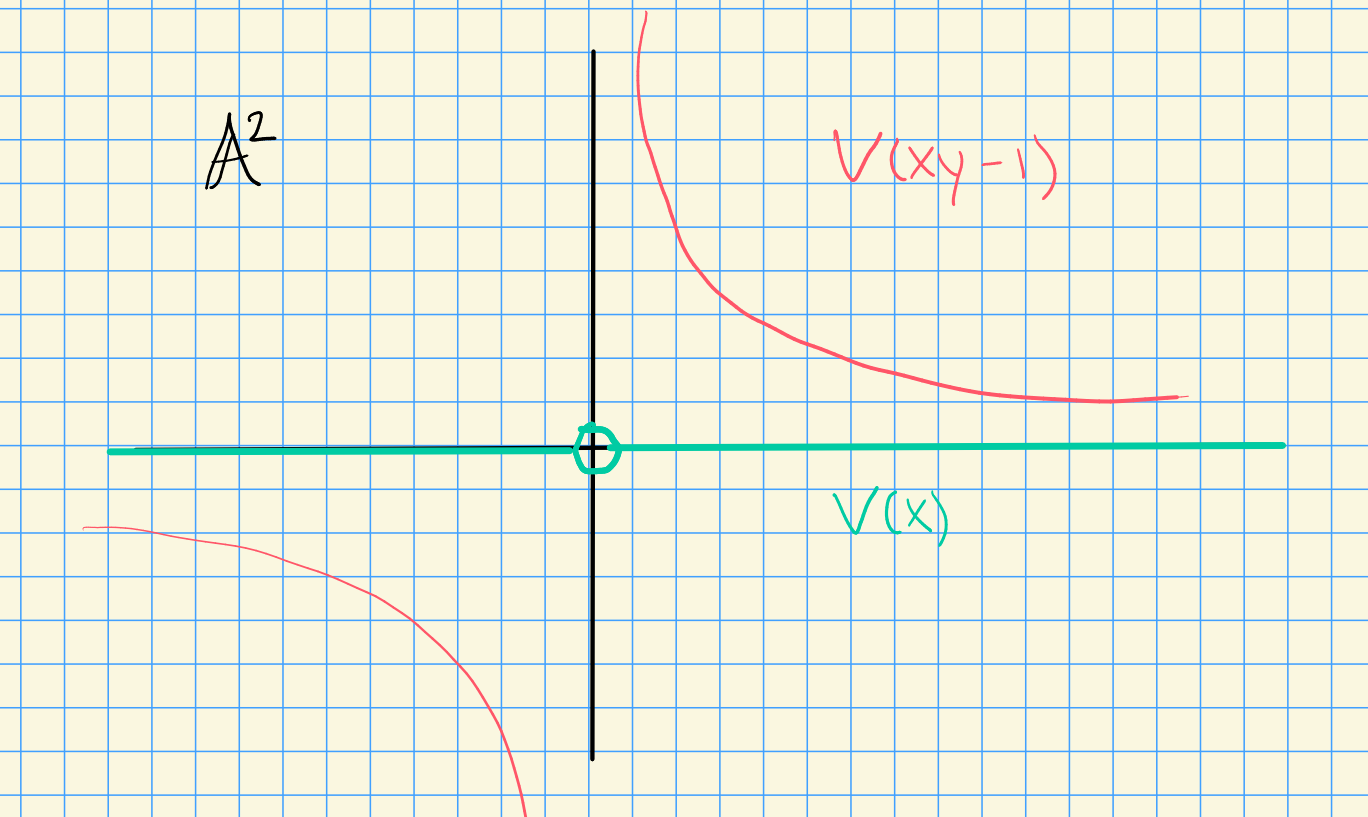
\includegraphics{figures/image_2020-10-15-09-50-03.png}
\caption{Image}
\end{figure}

Note that \(\pi: X\cross \AA^1 \to X\) is regular, using prop 3.8: if
the coordinates of a map are regular functions, then the entire map is a
morphism of ringed spaces. We can then note that \(1\over f(x)\) is
regular on \(D(f)\), since \(f\neq 0\) there.

\end{proof}

\begin{example}

\(\AA^2 \smz\) is not an affine variety. Note that this is also not a
distinguished open.

We showed on a HW problem that the regular functions on \(\AA^2\smz\)
are \(k[x, y]\), which are also the regular functions on \(\AA^2\). So
there is a map inducing a pullback
\begin{align*}  
\iota: \AA^2\smz &\to \AA^2 \\
\iota^* k[x, y] \mapsvia{\sim} k[x, y]
.\end{align*} Note that \(\iota^*\) is an isomorphism on the space of
regular functions, but \(\iota\) itself is not an isomorphism of
topological spaces. Why? \(i^{-1}\) is not defined at zero.

\end{example}

\hypertarget{chapter-5}{%
\subsection{Chapter 5}\label{chapter-5}}

\begin{definition}[Prevariety]

A \emph{prevariety} is a ringed spaced \(X\) with a finite open cover by
affine varieties. This is a topological space \(X\) with an open cover
\(\ts{U_i}_{i=1}^n \covers X\) such that \((U_i, \ro{\OO_X}{U_i} )\) is
isomorphic to an affine variety. We'll call \(\OO_X\) the sheaf of
\emph{regular functions} and \(U_i\subset X\) \emph{affine open sets}.

\end{definition}

One way to construct prevarieties from affine varieties is by
\emph{gluing}:

\begin{definition}[Glued Spaces]

let \(X_1, X_2\) be prevarieties which are themselves actual varieties.
Let \(U_{12} \subset X_1, U_{21} \subset X_2\) be opens and
\(f: U_{12} \to U_{21}\) an isomorphism of ringed spaces.

\begin{figure}
\centering
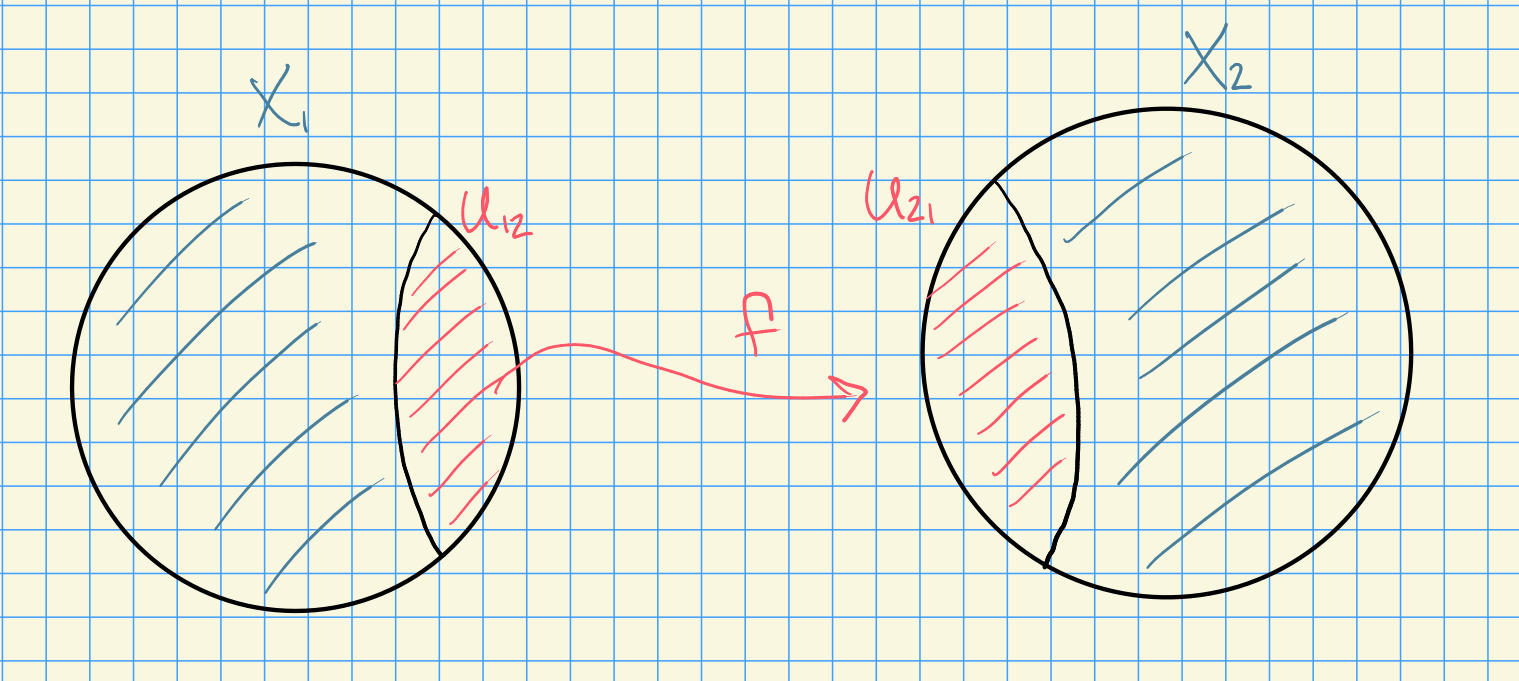
\includegraphics{figures/image_2020-10-15-10-08-59.png}
\caption{Image}
\end{figure}

As a set, take \(X = X_1 \disjoint X_2/\sim\) where \(a\sim f(a)\) for
all \(a\in U_{12}\). As a topological space, \(U \subset X\) is open iff
\(U_i \da U\intersect X_i\) are open in \(X_i\). As a ringed space, we
take
\(\OO_X(U) \da \ts{\phi: U\to k \st \ro{\phi}{U_i} \in \OO_{X_i}}\).

\end{definition}

\begin{example}

The prototypical example is \(\PP^1/k\) constructed from two copies of
\(\AA^1/k\). Set \(X_1 = \AA^1, X_2 = \AA^2\), with
\(U_{12} \da D(x) \subset X_1\) and \(U_{21} \da D(y) \subset X_2\).
Then let
\begin{align*}  
f: U_{12} &\to U_{21} \\
x & \mapsto {1\over x}
.\end{align*} This defines a regular function on \(U_{12}\) so defines a
morphism \(U_{12} \mapsvia{\sim} \AA^1\).

\begin{figure}
\centering
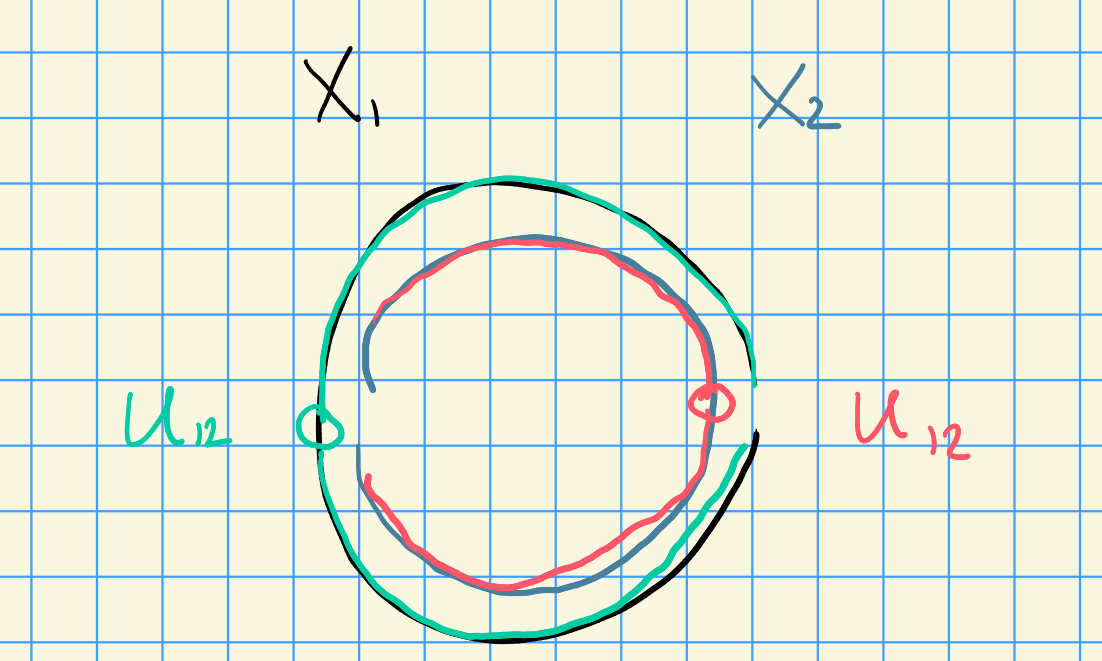
\includegraphics{figures/image_2020-10-15-10-20-32.png}
\caption{Image}
\end{figure}

Over \(\CC\), topologically this yields a sphere

\begin{figure}
\centering
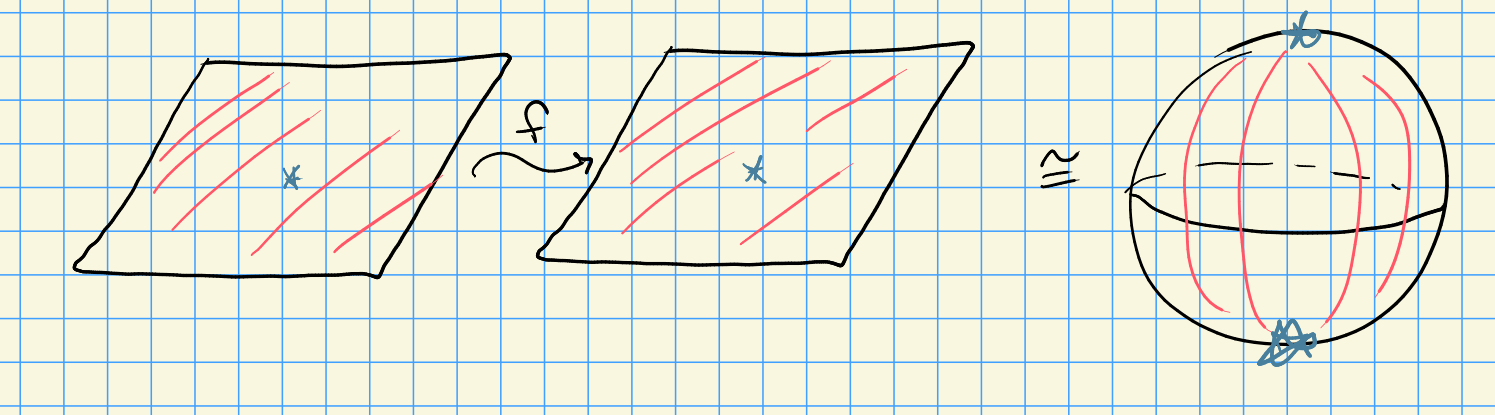
\includegraphics{figures/image_2020-10-15-10-23-24.png}
\caption{Image}
\end{figure}

Given a ringed space \(X = X_1\union X_2\) with a structure sheaf
\(\OO_X\), what is \(\OO_X(X)\)? By definition, it's

\begin{align*}  
\OO_X(X) \da \ts{\phi: X\to k \st \ro{\phi}{X_1}, \ro{\phi}{X_2} \text{ are regular} }
.\end{align*}

Then if \(\ro{\phi}{X_1} = f(x)\) and \(\ro{\phi}{X_2} = g(y)\), we have
\(y=1/x\) on the overlap and so \(\ro{f(x)}{D(x)} = \ro{g(1/x)}{D(x)}\).
Since \(f, g\) are rational functions agreeing on an infinite set,
\(f(x) = g(1/x)\) both being polynomial forces \(f = g = c\) for some
constant \(c \in k\). Thus \(\OO_X(X) = k\).

What about \(\OO_X(X_1)\)? This is just \(k[x]\), and similarly
\(\OO_X(X_2) = k[y]\). We can also consider
\(\OO_X(X_1\intersect X_2) = D(x) \subset X\), so this yields
\(k[x, 1/x]\). We thus have a diagram

\begin{center}\includesvg[width=\linewidth]{5c009219d6191466c14e5c66bc3eb7bbfb4aab01}\end{center}

\end{example}

\hypertarget{tuesday-october-20}{%
\section{Tuesday, October 20}\label{tuesday-october-20}}

\hypertarget{gluing-two-opens}{%
\subsection{Gluing Two Opens}\label{gluing-two-opens}}

Recall that a \emph{prevariety} is a ringed space that is locally
isomorphic to an affine variety, where we recall that \((X, \OO_X)\) is
\emph{locally isomorphic} to an affine variety iff there exists an open
cover \(U_i \covers X\) such that \((U_i, \OO_{U_i})\).

We found one way of producing these: the gluing construction. Given two
ringed spaces \((X_1, \OO_{X_1})\) and \((X_2, \OO_{X_2})\) and open
sets \(U_{12} \in X_1\) and \(U_{21} \in X_2\) and an isomorphism
\((U_{12}, \OO_{U_{12}}) \mapsvia{f} (U_{21}, \OO_{U_{21}})\), we
defined

\begin{itemize}
\tightlist
\item
  The topological space as \(X_1 \disjoint_f X_2\)
\item
  The sheaf of rings as
  \(\OO_X = \ts{\phi:U\to k \st\ro{\phi}{U\intersect X_i} \text{ is regular for } i=1,2 }\).
\end{itemize}

\begin{example}

\(\PP^1/k = X_1 \union X_2\) where \(X_1 \cong \AA^1, X_2 \cong \AA^2\).
Take \(U_{12} = D(x)\) and \(U_{21} = D(y)\) with
\begin{align*}  
f: U_{12} &\to U_{21} \\
x &\mapsto {1\over x} = y
.\end{align*}

\begin{figure}
\centering
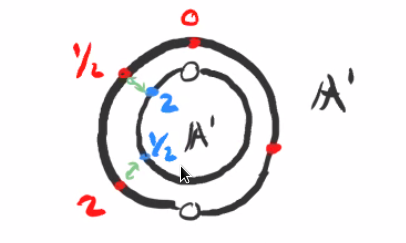
\includegraphics{figures/image_2020-10-20-09-41-55.png}
\caption{Supposing \(\ch(k) \neq 2\). Note that for \(\CC\) this
recovers \(S^2\) in the classical topology.}
\end{figure}

\end{example}

\begin{example}

Let \(X_i = \AA^1\) and \(U_{12} = D(x), U_{21} = D(y)\) with
\begin{align*}  
f: U_{12} &\to U_{21} \\
x &\mapsto x=y
.\end{align*}

\begin{figure}
\centering
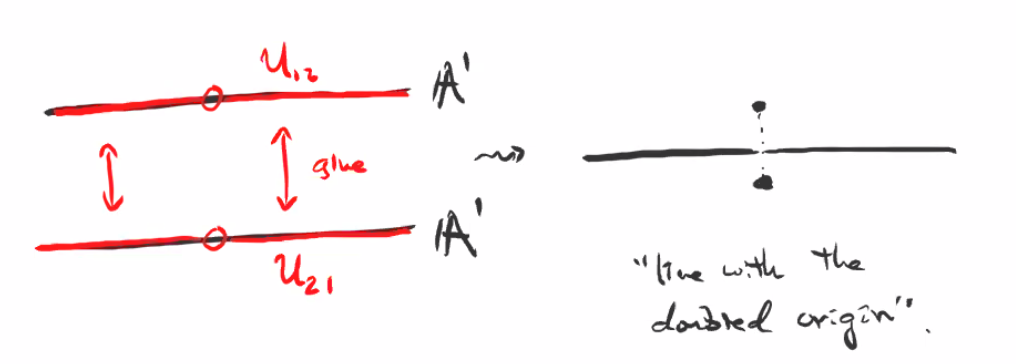
\includegraphics{figures/image_2020-10-20-09-44-41.png}
\caption{Line with the doubled origin.}
\end{figure}

Then
\(\OO_X = \ts{\phi: X\to k \st \ro{\phi}{X_i} \text{ is regular}} \cong k[x]\).

\end{example}

\hypertarget{more-general-gluing}{%
\subsection{More General Gluing}\label{more-general-gluing}}

Now we want to glue more than two open sets. Let \(I\) be an indexing
set for prevarieties \(X_i\). Suppose that for an ordered pair
\((i, j)\) we have open sets \(U_{ij} \subset X_i\) and isomorphisms
\(f_{ij}: U_{ij} \mapsvia{\sim} U_{ji}\) such that

\begin{enumerate}
\def\labelenumi{\alph{enumi}.}
\item
  \(f_{ji} = f_{ij}^{-1}\)
\item
  \(f_{jk} \circ f_{ij} = f_{ik}\) (cocycle condition)
\end{enumerate}

\begin{figure}
\centering
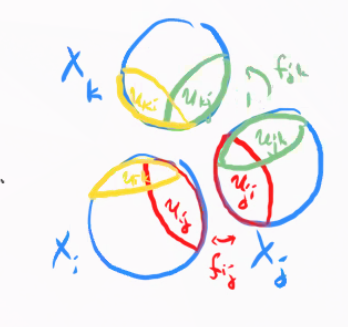
\includegraphics{figures/image_2020-10-20-09-54-14.png}
\caption{Opens with isomorphisms.}
\end{figure}

Then the gluing construction is given by

\begin{enumerate}
\def\labelenumi{\arabic{enumi}.}
\item
  \(X\da \disjoint X_i/\sim\) where \(x\sim f_{ij}(x)\) for all \(i,j\)
  and all \(x\in U_{ij}\).
\item
  \(\OO_x(U) \da \ts{\phi:U\to k \st \ro{\phi}{U\intersect X_i} \in \OO_{X_i} }\).
\end{enumerate}

Every prevariety arises from the gluing construction applied to \(X_i\)
affine varieties, since a prevariety \((X, \OO_X)\) by definition has an
open affine cover \(X_i \covers X\) and \(X\) is the result of gluing
the \(X_i\)s by the identity.

\begin{example}

Let \(X_1 = X_2 = X_3 = \AA^2/k\). Glue by the following instructions:

\begin{figure}
\centering
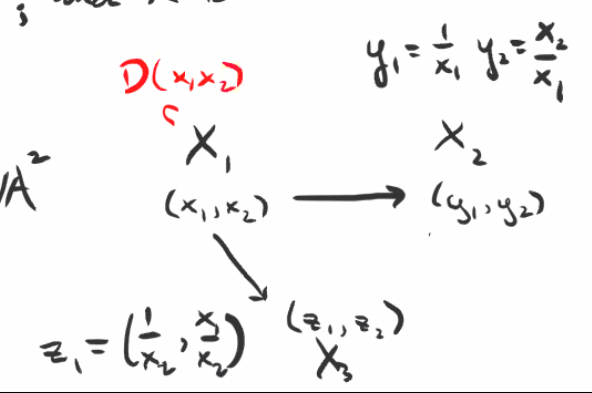
\includegraphics{figures/image_2020-10-20-10-11-07.png}
\caption{The map not shown is whatever formula is necessary to make the
diagram commute.}
\end{figure}

Here

\begin{itemize}
\tightlist
\item
  \((y_1, y_2) = (1/x_1, x_2/x_1)\)
\item
  \((z_1, z_2) = (1/x_2, x_1/x_2)\)
\item
  \(U_{12} = D(x_1)\)
\item
  \(U_{21} = D(x_2)\).
\end{itemize}

\begin{figure}
\centering
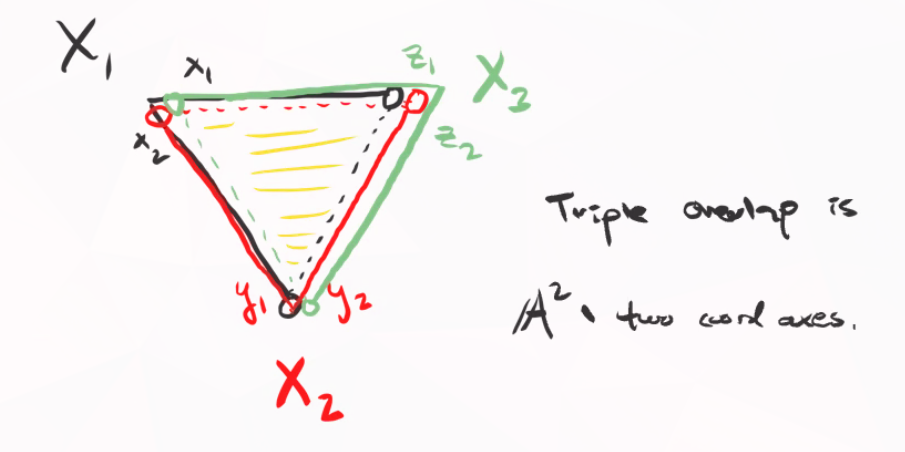
\includegraphics{figures/image_2020-10-20-10-13-56.png}
\caption{Yields \(\PP^2\)}
\end{figure}

Here \(X_1 = [1: y/x: z/x]\), \(X_2 = [x/y: 1: z/y]\).

\end{example}

\begin{example}

From Gathmann 5.10, open and closed subprevarieties. Let \(X\) be a
prevariety and suppose \(U\subset X\) is open. Then \((U, \OO_U)\) is a
prevariety where \(\OO_U = \ro{\OO_X}{U}\). How can we write \(U\) as
(locally) an affine variety?

Since the \(U_i\) are covered by distinguished opens \(D_{ij}\) in
\(X_i\) where \(X = \union X_i\) with \(X_i\) affine varieties, we can
write \(U = \Union_i U_i = \Union_{i, j} D_{ij}\).

\end{example}

\begin{example}

Let \(Y\subset X\) be a closed subset of a prevariety \(X\). We need to
define \(\OO_Y(U)\) for all \(U\subset Y\) open, so we set
\begin{align*}  
\OO_Y(U) = \ts{\phi: U\to k \st \forall p\in U, \, \exists V_p \text{ with } p\in V_p \subset_{\text{open}} X \text{ and } \psi\in \OO_X(V_p) \text{ s.t. } \ro{\psi}{U\intersect V} \phi  }
.\end{align*}

What's the picture?

\begin{figure}
\centering
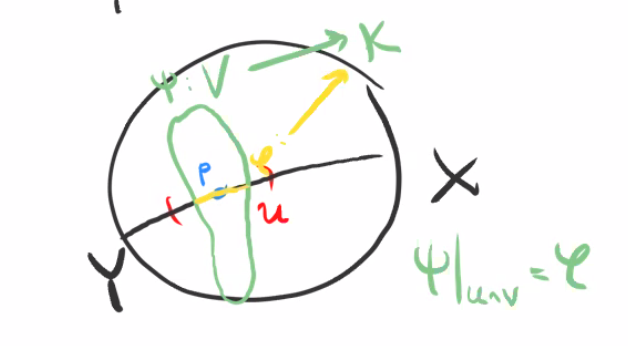
\includegraphics{figures/image_2020-10-20-10-29-25.png}
\caption{Sheaf for a closed subset.}
\end{figure}

It's an exercise to show that this is a prevariety.

\end{example}

\begin{remark}

If \(U\subset X\) is an open subprevariety or \(Y\subset X\) is a closed
subprevariety, then the inclusions are morphisms. We'd need to show that
a pullback of a function is regular, but this is set up by definition.

\end{remark}

\begin{remark}

Define \(\tilde \OO_X(U)\) as the set of \emph{all} functions
\(U\to k\). Then the inclusion \((X, \OO_X) \injects (X, \tilde \OO_X)\)
given by the identity on \(X\) is a morphism, but the identity in the
reverse direction is not.

\end{remark}

\hypertarget{misc-unsorted}{%
\section{Misc Unsorted}\label{misc-unsorted}}

\begin{figure}
\centering
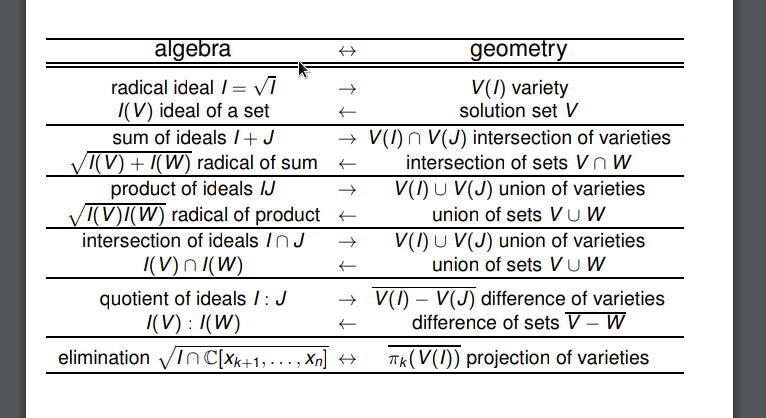
\includegraphics{figures/image_2020-09-16-04-09-22.png}
\caption{Image}
\end{figure}

\newpage

\section{Indices}
\newpage
\listoftodos[List of Todos]

% Hook into amsthm environments to list them.
\renewcommand{\listtheoremname}{Definitions}
\listoftheorems[ignoreall,show={definition}, numwidth=3.5em]

\renewcommand{\listtheoremname}{Theorems}
\listoftheorems[ignoreall,show={theorem,proposition}, numwidth=3.5em]

\renewcommand{\listtheoremname}{Exercises}
\listoftheorems[ignoreall,show={exercise}, numwidth=3.5em]

\listoffigures



\printbibliography[title=Bibliography]


\end{document}
